%% Based on a TeXnicCenter-Template, which was
%% created by Christoph B�rensen
%% and slightly modified by Tino Weinkauf.
%%%%%%%%%%%%%%%%%%%%%%%%%%%%%%%%%%%%%%%%%%%%%%%%%%%%%%%%%%%%%

\documentclass[a4paper,12pt]{scrartcl} %This is a special class provided by the KOMA script, which does a lot of adjustments to adapt the standard LaTeX classes to european habits, change to [a4paper,12pt,twoside] for doublesided layout


%########################### Preferences #################################

% ******** vmargin settings *********
\usepackage{vmargin} %This give you full control over the used page arae, it maybe not the idea od Latex to do so, but I wanted to reduce to amount of white space on the page
\setpapersize{A4}
\setmargins{2.2cm}%     %linker Rand, left edge
					 {1.4cm}%     %oberer Rand, top edge
           {16.7cm}%    %Textbreite, text width
           {24.2cm}%    %Texthoehe, text hight
           {14pt}%      %Kopfzeilenh�he, header hight
           {1cm}%       %Kopfzeilenabstand, header distance
           {0pt}%       %Fu�zeilenhoehe footer hight
           {2cm}%       %Fusszeilenabstand, footer distance         

% ********* Font definiton ************
\usepackage{t1enc} % as usual
\usepackage[latin1]{inputenc} % as usual
\usepackage{times}		
\usepackage[T1]{fontenc}
\usepackage{amsfonts,amssymb,amsmath}
\usepackage{url}
\usepackage[dvipsnames,usenames]{color}
\usepackage{multirow}


\def\courierFive   {\fontfamily{pcr}\fontsize{5.0}{ 6.25pt}\selectfont}
\def\courierSix    {\fontfamily{pcr}\fontsize{6.0}{ 7.50pt}\selectfont}
\def\courierSeven  {\fontfamily{pcr}\fontsize{7.0}{ 8.75pt}\selectfont}
\def\courierEight  {\fontfamily{pcr}\fontsize{8.0}{10.00pt}\selectfont}
\def\courierNine   {\fontfamily{pcr}\fontsize{9.0}{11.25pt}\selectfont}
\def\courier       {\fontfamily{pcr}\selectfont}

\newcommand{\courierNineMakeTenPowX}[1]{\ensuremath{\times}{\courierNine 10}\ensuremath{^{\text{\courierSeven{#1}}}}}


\def\efloat          {e{\ttfamily\underline\ }float}
\def\efloatbase      {e{\ttfamily\underline\ }float{\ttfamily\underline\ }base}
\def\efloatbaseclass {{\courier{e{\ttfamily\underline\ }float{\ttfamily\underline\ }base}}}
\def\efloatclass     {{\courier{e{\ttfamily\underline\ }float}}}
\def\efxefloatclass  {{\courier{efx::e{\ttfamily\underline\ }float}}}
\def\mpfrefloatclass {{\courier{mpfr::e{\ttfamily\underline\ }float}}}
\def\gmpefloatclass  {{\courier{gmp::e{\ttfamily\underline\ }float}}}
\def\forefloatclass  {{\courier{f90::e{\ttfamily\underline\ }float}}}
\def\efcomplexclass  {{\courier{ef{\ttfamily\underline\ }complex}}}

\def\efloathyperref     {\texorpdfstring{\efloat}{e\_float}}
\def\efloatbasehyperref {\texorpdfstring{\efloatbase}{e\_float\_base}}


\def\mathematica {Math\-e\-ma\-tica{\footnotesize {\textregistered}}}

\renewcommand\Re{\operatorname{\mathfrak{Re}}}
\renewcommand\Im{\operatorname{\mathfrak{Im}}}


% ********* Graphics definition *******
\usepackage[pdftex]{graphicx} % required to import graphic files
\usepackage[dvipsnames,usenames]{color}
\usepackage{eso-pic} % these two are required to add the little picture on top of every page
\usepackage{everyshi} % these two are required to add the little picture on top of every page
\renewcommand{\floatpagefraction}{0.7} %default:0.5 allows two big pictures on one page

% ********* Source code highlighting *******
\usepackage{listings}
\usepackage{textcomp}

\definecolor{CodeBackgroundColor}{rgb}{0.90,0.90,0.90}
\definecolor{IdentifyerColor}{rgb}{0.10,0.10,0.50}

\def\lstsetCPlusPlus{
\lstset{
language=[ISO]C++,
  keywordstyle=\bfseries\courier\color[rgb]{0,0,1},
  identifierstyle=\color{IdentifyerColor},
  commentstyle=\itshape\color{OliveGreen},
  stringstyle=\color{BrickRed},
  showstringspaces=false,
  basicstyle=\courierEight,
  numberstyle=\tiny,
  numbers=left,
  stepnumber=1,
  numbersep=6pt,
  tabsize=2,
  breaklines=true,
  prebreak = \raisebox{0ex}[0ex][0ex]{\ensuremath{\hookleftarrow}},
  breakatwhitespace=false,
  aboveskip={1.5\baselineskip},
  columns=fixed,
  upquote=true,
  extendedchars=true,
  frame=tlrb,
  backgroundcolor=\color{CodeBackgroundColor},
}
}

\def\lstsetBash{
\lstset{
  language=bash,
  basicstyle=\ttfamily,
  keywordstyle=\ttfamily,
  frame=tlrb,
  backgroundcolor=\color{CodeBackgroundColor},
}
}

%********** Enable Hyperlinks *******
\usepackage[pdfborder=000,pdftex=true]{hyperref}% this enables jumping from a reference and table of content in the pdf file to its target

% ********* Table layout **************
\usepackage{booktabs}	  	%design of table, has an excellent documentation
%\usepackage{lscape}			%use this if you want to rotate the table together with the lines around the table

% ********* Caption Layout ************
\usepackage{ccaption} % allows special formating of the captions
\captionnamefont{\bf\footnotesize\sffamily} % defines the font of the caption name (e.g. Figure: or Table:)
\captiontitlefont{\footnotesize\sffamily} % defines the font of the caption text (same as above, but not bold)
\setlength{\abovecaptionskip}{0mm} %lowers the distace of captions to the figure


% ********* Header and Footer **********
% This is something to play with forever. I use here the advanced settings of the KOMA script

\usepackage{scrpage} %header and footer using the options for the KOMA script
\renewcommand{\headfont}{\footnotesize\sffamily} % font for the header
\renewcommand{\pnumfont}{\footnotesize\sffamily} % font for the pagenumbers

%the following lines define the pagestyle for the main document
\defpagestyle{cb}{%
(\textwidth,0pt)% sets the border line above the header
{\pagemark\hfill\headmark\hfill}% doublesided, left page
{\hfill\headmark\hfill\pagemark}% doublesided, right page
{\hfill\headmark\hfill\pagemark}%  onesided
(\textwidth,1pt)}% sets the border line below the header
%
{(\textwidth,1pt)% sets the border line above the footer
{{\it e\underline float@yahoo.com}\hfill Christopher Kormanyos}% doublesided, left page
{Christopher Kormanyos\hfill{\it e\underline\ float@yahoo.com}}% doublesided, right page
{Christopher Kormanyos\hfill{\it e\underline\ float@yahoo.com}} % one sided printing
(\textwidth,0pt)% sets the border line below the footer
}

%this defines the page style for the first pages: all empty
\renewpagestyle{plain}%
	{(\textwidth,0pt)%
		{\hfill}{\hfill}{\hfill}%
	(\textwidth,0pt)}%
	{(\textwidth,0pt)%	
		{\hfill}{\hfill}{\hfill}%
	(\textwidth,0pt)}

%********** Footnotes **********
\renewcommand{\footnoterule}{\rule{5cm}{0.2mm} \vspace{0.3cm}} %increases the distance of footnotes from the text
\deffootnote[1em]{1em}{1em}{\textsuperscript{\normalfont\thefootnotemark}} %some moe formattion on footnotes

%################ End Preferences, Begin Document #####################

\pagestyle{plain} % on headers or footers on the first page

\begin{document}

% There might be better solutions for the title page, giving all distances
% and sizes manually was simply the easiest solution

\begin{center}

{\Huge\bf\sf \efloat\ User's Manual}

\vspace{2cm}

{\Large\bf\sf Christopher Kormanyos}%as this is an english text I didn't load the german package, this would ease the use of special characters
\vspace{2cm}

{\Large\bf\sf Version 1.0 from \today} %adds the current date

\vspace{\fill}

e\underline\ float@yahoo.com

\end{center}

\newpage

%%The following loads the picture on top of every page, the numbers in \put() define the position on the page:
%\AddToShipoutPicture{\setlength\unitlength{0.1mm}\put(604,2522){\includegraphics[width=1.5cm]{logo.jpg}}}

\pagestyle{cb} % now we want to have headers and footers

\tableofcontents

\newpage

\section   {About \efloathyperref}                   \label{sec:about}
                                                     \subsection{Introduction}

There are many multiple precision (MP) packages available to
the scientific and engineering community.
Each package has individual strengths within its range
of application. However, most MP packages lack a uniform interface
for high precision algorithm design. They also offer little or
no special function support. Also, many MP packages have
limited portability. There is no portable standalone C++ system
which offers a wide variety of high precision special functions
and handles large function parameters.

The \efloat\ system (extended float) not only addresses these weaknesses
but also significantly advances MP technology. It uses several 
MP packages and provides a uniform C++ interface for high precision
algorithm design, independent of the underlying MP implementation.
In addition, \efloat\ supports a large collection
of high performance MP functions which are
entirely portable, solidly designed and can be used with any
suitably prepared MP type. Furthermore, the \efloat\ system
provides software interfaces for seamless interoperability
with other high level languages.
No MP system other than \efloat\ offers such a high degree
of portability, such a wide range of functions, and such
a rich selection of powerful interoperabilities.
The \efloat\ library can be used for a variety of
purposes such as high precision function evaluation,
numerical verification of compilers, function libraries or
other computational systems as well as investigations of
compiler quality, optimization methods and computer hardware.

\efloat\ is unique because it is designed from the ground up utilizing
generic and object--oriented design methods to create an efficient and
flexible numerical software architecture
\cite{coplien:textbook}, \cite{vandevoorde:textbook}, \cite{yang:textbook}.
The standard containers and algorithms of the C++ STL and TR1 are
consistently used to reduce programmatic complexity \cite{becker:textbook},
\cite{isoiec14882:textbook}, \cite{isoiec19768:textbook}, \cite{josuttis:textbook}.
Static and dynamic polymorphism are used to implement a standardized
interface to MP types allowing for the interchangeable use of different
MP implementations.

\efloat\ is written in the C++ language making broad use of the
C++ core language, much of the STL and some of TR1,
as specified in ISO/IEC 14882:2003
and ISO/IEC 19768:2007 \cite{isoiec14882:textbook,isoiec19768:textbook}.
It is emphasized that the C++ compiler must closely adhere to
these standards in order to successfully compile and link \efloat.
The source codes have been implemented according to safe programming
practices and reliability standards originating from the automotive industry
\cite{misra:misrac,misra:misracpp}.
A great effort has been invested in advanced C++ optimization techniques
in order to improve system performance.
Generic and object--oriented programming methods have been used
to create an efficient and flexible numerical software architecture.
In addition, consistent use of standard containers and algorithms of the
STL and TR1~\cite{josuttis:textbook,becker:textbook} has significantly
reduced and evenly distributed the computational complexities
of the entire program.

Advanced programming techniques have been used to implement
interfaces to other high level languages, including the
Microsoft{\footnotesize {\textregistered}}~CLR,
Python, Iron\-Python and Wolfram's \mathematica\
(see \cite{isoiec23271:textbook,microsoft:clr,python:website,foord:textbook,ironpython:website,wolfram:textbook}).
This means that it is possible to combine the calculating power of several systems
to obtain a hybrid system which is more powerful than either one of its parts.
For example, \efloat\ can be used with the C\# language~\cite{isoiec23270:textbook},
targeting the CLR in the
Microsoft{\footnotesize {\textregistered}}.NET Framework.
This exposes the efficient calculating power of \efloat\ to the high level
graphical--user--interface (GUI) design regime of C\# in the CLR.
At the same time the GUI design is separated from complex MP algorithms.
This is a very powerful hybrid system based on effective distribution of
computational complexity.

The \efloat\ software project consists of approximately 110 manually written
source files with $\sim$20,000 lines of code in addition to about 20 automatically
generated files with $\sim$200,000 lines of code.
The source codes of \efloat\ are implemented in accordance with safe programming
practices and reliability standards originating from the automotive industry
\cite{misra:misrac}, \cite{misra:misracpp}.

The \efloat\ source code is released under the `Boost Software License' (BSL)
from boost \cite{boostlic:website}. Unlike the the `General Public License' (GPL)
from GNU \cite{gnulic:website}, the BSL permits the creation of works derived from \efloat\
for any commercial, or non-commercial, or non-profit use with no legal requirement
to release the \efloat\ source code \cite{boostlic:website}.

\subsection{Configurations}

\begin{table}[h]\noindent
\begin{center}
\renewcommand{\arraystretch}{1.05}
\begin{tabular}{c|c|c|c}

Config
            & \efloatclass\ Class
            & Capabilities
            & Dependencies \\

\hline

\multirow{2}{*}{efx}
            & \multirow{2}{*}{\efxefloatclass}
            & functions, algorithm design,
            & \multirow{2}{*}{---} \\

\ %space
            & \ %space
            & test and benchmark
            & \\

\hline

gmp
            & \gmpefloatclass\
            & ''$\quad\quad$''
            & GMP library \\

\hline

\multirow{2}{*}{mpfr}
            & \multirow{2}{*}{\mpfrefloatclass}
            & \multirow{2}{*}{''$\quad\quad$''}
            & GMP library, \\

\ %space
            & \ %space
            & \ %space
            & MPFR library \\

\hline

\multirow{2}{*}{f90}
            & \multirow{2}{*}{\mpfrefloatclass}
            & \multirow{2}{*}{''$\quad\quad$''}
            & {\courier{REAL(KIND\ensuremath{=}16)}} wrap, \\

\ %space
            & \ %space
            & \ %space
            & Fortran run--time libraries \\

\hline

\multirow{3}{*}{pyd}
            & \multirow{3}{*}{any \efloatclass}
            & functions, algorithm design,
            & those of its {\courier{e{\ttfamily\underline\ }float}} type, \\

\ %space
            & \ %space
            & rapid prototyping,
            & {\courier{boost.python}} library, \\

\ %space
            & \ %space
            & high level Python scripting
            & Python library \\

\hline

\multirow{4}{*}{clr}
            & \multirow{4}{*}{any \efloatclass}
            & functions, algorithm design,
            & \ \\

\ %space
            & \ %space
            & rapid prototyping,
            & those of its {\courier{e{\ttfamily\underline\ }float}} type, \\

\ %space
            & \ %space
            & high level scripting,
            & common language runtime \\

\ %space
            & \ %space
            & CLR GUI development
            & \ \\

\hline


\multirow{2}{*}{cas}
            & \multirow{2}{*}{any \efloatclass}
            & \multirow{2}{*}{computer algebra interoperability}
            & those of its {\courier{e{\ttfamily\underline\ }float}} type, \\

\ %space
            & \ %space
            & \ %space
            & computer algebra system \\

\hline
\end{tabular}
\vspace{2.0mm}
\caption{The system configurations of \efloat\ are shown.}
\label{table:systemconfigs}
\end{center}
\end{table}



The \efloat\ system supports a variety of configurations
using several \efloatclass\ classes
as well as other libraries and systems.
These are shown in Table~\ref{table:systemconfigs}.
Details about the capabilities and dependencies of the
configurations are also included in the table.

\pagebreak

\subsection{The \efloathyperref\ System Architecture}\label{sec:architecture}

\begin{figure*}[p]
\centering
\framebox{\hspace{2.0mm}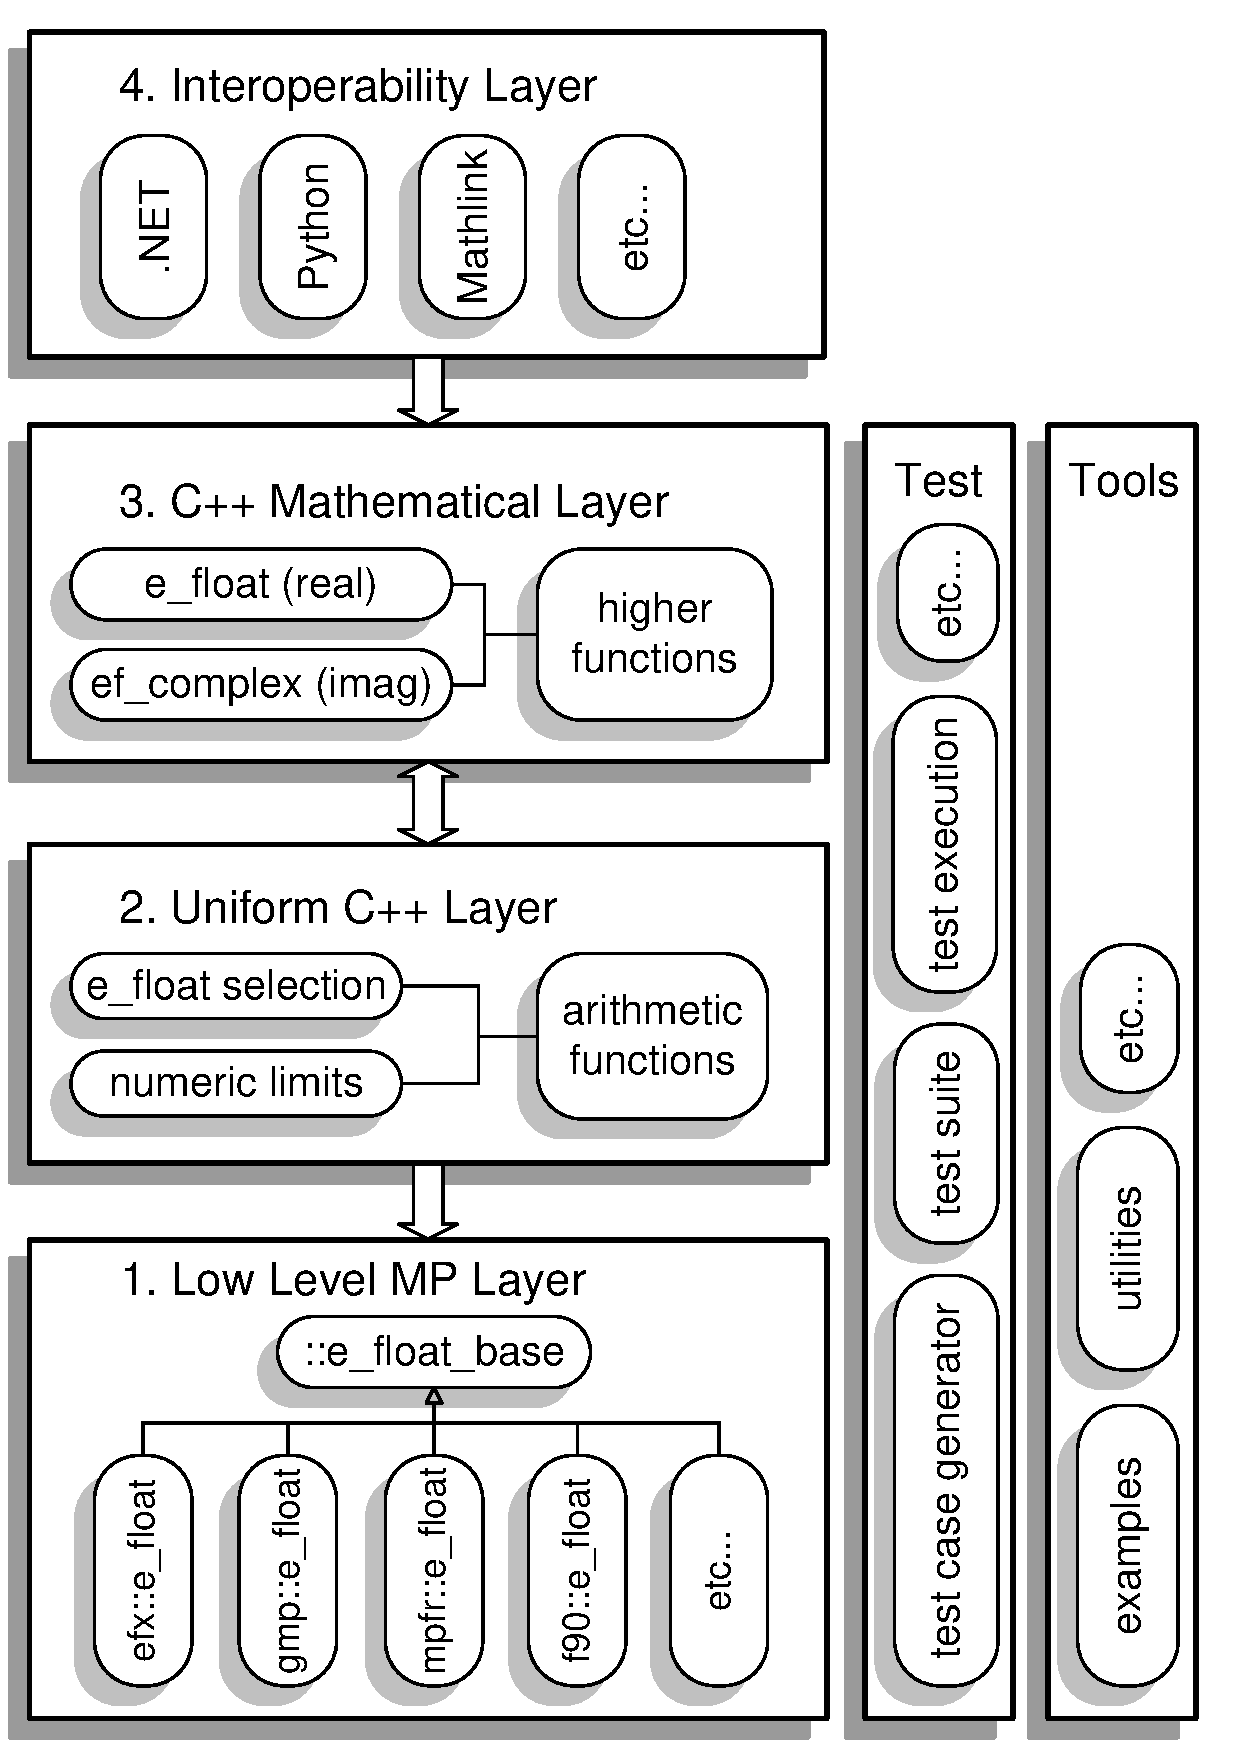
\includegraphics[width=16.0cm]{e_float_architecture.pdf}}
\vspace{2.0mm}
\caption{The \efloat\ system architecture is shown.}
\label{figure:architecture}
\end{figure*}

The \efloat\ system architecture is robust and flexible.
With this architecture, both the integration of other MP types as well as
the addition of more functions and interoperabilities can be done with ease. 
The system architecture is shown in Figure~\ref{figure:architecture}.
It has four layers and two additional
blocks, the test block and the tools block. Layers $1$--$4$ have successively
increasing levels of abstraction. They build up very high level
functionalities in a stable, stepwise fashion.
Note that ``{\emph e}{\ttfamily{\underline\ }}{\emph{float}}''
is not only the name of the system but also the name of several
\efloatclass\ classes.

Layer~$1$, the low level MP layer, ensures that each
implementation--dependent, possibly non--portable MP implementation
is suitably prepared to conform with the C++ class requirements of Layer~$2$.
Each individual MP type is encapsulated within a specific
\efloatclass\ C++ class,
each one of which defined within its own unique name\-space.
For example, classes such as
{\courier{efx::e{\ttfamily\underline\ }float}},
{\courier{gmp::e\underline\ float}} and others are implemented.
Each of these classes is derived from a common abstract
base class called {\courier{::e{\ttfamily\underline\ }float{\ttfamily\underline\ }base}}.
The abstract base class defines public and pure virtual functions
which implement arithmetic primitives such as self--multiplication,
self--compare, special numbers like NaN, and string operations.
These arithmetic primitives fulfill the requirements necessary for
elementary mathematics. They simultaneously conform with Layer~$2$.
Thus, via inheritance and implementation of virtual functions,
each individual \efloatclass\
class supports elementary mathematics and also complies with Layer~$2$.

Some MP types include their own versions of various functions.
Layer~$1$ accommodates this with the
``{\emph{has--its--own}}''--mechanism. This mechanism allows the
C++ interface of a given MP type to use the MP's own
algorithm for a particular function.
It uses virtual Boolean functions prefixed with
``{\courier{has{\ttfamily\underline\ }its{\ttfamily\underline\ }own}}''.
For example,
{\courier{has{\ttfamily\underline\ }its{\ttfamily\underline\ }own{\ttfamily\underline\ }sin}}
returns {\courier{true}} in order to use the MP's own implementation
of $\sin(x)$, $x$$\,\in$$\,\mathbb{R}$.
The performance of a specific MP class can be optimized
by selectively activating these functions.
MPFR~\cite{33:2:1} has its own implementations of most elementary functions
and several higher transcendental functions. The elementary functions
are quite efficient and these are, in fact, used to optimize the
performance of {\courier{mpfr::e{\ttfamily\underline\ }float}}.

Layer~$2$ implements the uniform C++ interface.
The \efloatclass\ type from layer~$1$, which will be used in the
project configuration, is selected with a
compile--time option. The functions of this \efloatclass\
class are used to implement all arithmetic operations,
numeric limits and basic I/O mechanisms.
Thus, layer~$2$ provides a uniform C++ interface which is
generic and fully equipped with all the basic functions
necessary for high level MP algorithm design in a C++ environment.

Layer~$3$ is the C++ mathematical layer.
It adds the class {\courier{ef{\ttfamily\underline\ }complex}},
{\emph{i.e.}} the complex data type. 
This layer uses both the selected \efloatclass\
type as well as {\courier{ef{\ttfamily\underline\ }complex}}
to implement \efloat 's rich collection of elementary functions and higher
transcendental functions.

Layer~$4$, the interoperability user layer, exposes all of the
functions and capabilities of layers~$2$ and $3$ to other
high level languages. Marshaling techniques~\cite{richterclr:textbook}
are used to create managed C++ classes and wrapper functions
which embody the full functionality of layers~$2$ and $3$.
These are compiled to a single CLR assembly which can be used with
all Microsoft{\footnotesize {\textregistered}} CLR
languages including C\#, managed C++/CLI, Iron\-Python, {\emph{etc}}.
Compatibility with the
Microsoft{\footnotesize {\textregistered}}.NET Framework~$3$.$5$ has been tested.
Another interoperability employs the {\courier{boost.py\-thon}}
library~\cite{boostpython:website} to
expose the functionality of layers~$2$ and $3$ to Python.
Compatibilities with Python~$2$.$6$.$4$ and boost~$\geq\,1$.$39$
have been tested.

Another layer~$4$ interoperability targets \mathematica.
A sparse architecture has been developed to create a generic interface
for interacting with computer algebra systems. The compatibility
of this interface with \mathematica~$7$.$1$ has been tested.
The interoperabilities of layer~$4$ are very powerful mechanisms
based on highly advanced programming techniques.
They can be used for very high level designs such as
scripting, rapid algorithm prototyping and result visualization.

The test block contains several hundred automatically
generated test files which have been specifically designed to test all
algorithms and convergence regions of the entire \efloat\ system.
The test block includes an automatic test execution system and an automatic
test case generator. This block allows for fully reproducible automated
testing of the system.

The tool block contains a variety of utilities and examples.
The utilities predominantly consist of generic templates
for standard mathematical operations such as numerical differentiation,
root finding, recursive quadrature, {\emph{etc}}.
The examples show practical, non--trivial
uses of the \efloat\ system involving both high level algorithm design
as well as interoperability.

The \efloat\ architecture exemplifies how layered
design can be leveraged to find the right granularity to distribute
a very large computational complexity among smaller constituents
which have manageable software scope.
For example, there are vast software distances
between the hand--optimized assembler routines of
GNU MP~\cite{gmp:website} and, for example, the Hurwitz zeta function,
or a high level GUI in C\#.
The \efloat\ architecture elegantly navigates
these distances to build up high level functionalities in
a controlled, stepwise fashion.

The \efloat\ system architecture is a significant technological
milestone in MP programming technology. While other MP packages do sometimes
provide a specialized C++ interface for their own specific implementations,
they are mostly incompatible with each other.
However, \efloat 's uniform C++ layer creates a
generic interface which can be used with any underlying MP type.
Assuming that a given MP type can be brought into conformance with layer~$2$,
it can be used in a portable fashion with all of \efloat 's capabilities
including arithmetic, elementary functions, special functions, interoperabilities,
automatic tests, utilities, and additional user--created extensions.

\pagebreak

\subsection{MP Types}

\begin{table}[ht]\noindent
\begin{center}
\renewcommand{\arraystretch}{1.20}
\begin{tabular}{c|l|c|c}

Class Name
            & Internal Representation
						& Digits
						& Padding \\

\hline

\multirow{4}{*}{{\courier{efx::e{\ttfamily\underline\ }float}}}
            & data: {\courier{UINT32}} base--$10^{8}$ array
						& \multirow{4}{*}{$30$--$300$}
						& \multirow{4}{*}{$15$\%} \\

\ %space
            & Boolean negative sign
            & \ %space
						& \ \\

\ %space
            & {\courier{INT64}} base--10 exponent
            & \ %space
						& \ \\

\ %space
            & floating point class (finite, NaN, {\emph{etc}}.)
            & \ %space
						& \ \\

\hline

\multirow{2}{*}{{\courier{gmp::e{\ttfamily\underline\ }float}}}
            & data: GMP's type {\courier{::mpf{\ttfamily\underline\ }t}}
						& \multirow{2}{*}{$30$--$300$}
						& \multirow{2}{*}{$15$\%} \\

\ %space
            & floating point class (finite, NaN, {\emph{etc}}.)
            & \ %space
						& \ \\

\hline

{\courier{mpfr::e{\ttfamily\underline\ }float}}
            & data: MPFR's type {\courier{::mpfr{\ttfamily\underline\ }t}}
						& $30$--$300$
						& $15$\% \\

\hline

{\courier{f90::e{\ttfamily\underline\ }float}}
            & data: Fortran's type {\courier{REAL(KIND\ensuremath{=}16)}}
						& $\sim$$\,30$
						& $4$--$5$ digits \\

\hline

\end{tabular}
\vspace{2.0mm}
\caption{The MP classes in \efloat\ are shown. Details about the internal representation
as well as the digit range and the added internal extra digits ({\emph{i.e.}} the padding) are given.}
\label{table:mpclasses}
\end{center}
\end{table}



Four MP types have been selected for inclusion in \efloat.
These are listed in Table~\ref{table:mpclasses}.
The table also includes information about the internal
representations of the individual MP classes and
their digit ranges.
The three main \efloatclass\ classes are
\efxefloatclass, \mpfrefloatclass\ and \gmpefloatclass.
They are designed for high precision calculations with large
exponent range.

GNU MP and MPFR have been included
because of their high performance, their general acceptance
in the scientific community and their widespread availability
(at least for Unix/Linux--GNU systems). Unfortunately,
these libraries are not easily ported to compiler and
build systems other than GCC and GNU\-make.
However, for the \efloat\ development GNU MP~$4$.$2$.$4$
and MPFR~$2$.$4$.$1$ have been ported to
Microsoft{\footnotesize {\textregistered}}
Visual Studio{\footnotesize {\textregistered}} 2008,
based in part on Glad\-man's~\cite{gladman:ports} port.

A new MP type called EFX, {\emph {extended--float--x}}, has been created for
the \efloat\ system. It is written entirely in C++ and uses
base--$10^{8}$ data elements. Since GNU MP and MPFR use more
efficient base--$2^{n}$ data elements and because they take advantage
of hand--optimized assembler for the most time--critical inner loops,
EFX does not quite reach the performance of either GNU MP or MPFR.
However, EFX has other advantages --- a base--$10$ representation as
well as a data field which is created on the stack, not using dynamic
memory allocation. Therefore, the base--10 numerical value can be viewed
in a human recognizable form with a graphical debugger,
without awkward print operations or code modifications.
This makes EFX well suited for algorithm development. EFX has been used
for all early algorithm prototyping during the \efloat\ development.

The final MP type is called F90. It uses a skinny For\-tran~$90$/C++
layer to wrap the Fortran quadruple--precision data type
{\courier{REAL(KIND\ensuremath{=}16)}}.
The range of this MP type is limited to that of
the Fortran type --- about 30 digits of precision with an exponent
of about $\pm\,4000$. Due to its limited range, \forefloatclass\
only passes about $75$\% of the test cases defined in
the test suite. If this range sufficient
for the application, then \forefloatclass\ is extremely fast
because it uses a native data type.




\pagebreak

\section   {Building \efloathyperref}                \label{sec:build}
                                                     
Every effort has been made to ensure that building
the \efloat\ system is straightforward.
The default build supports execution of the test suite
with the selected \efloatclass\ type.
Simple operations or other spot--tests can be carried out by deactivating
the subroutine
{\courier{::test{\ttfamily{\underline\ }}real{\ttfamily{\underline\ }}imag}}
and activating the subroutine
{\courier{test::spot::test{\ttfamily{\underline\ }}spot}}
in the {\courier main} program which is implemented in the
file {\courier {test/test.cpp}}.
Designers of advanced applications can remove the test suite entirely
and create a custom build.

\subsection{Compiler Systems}

\begin{table}[ht]\noindent
\begin{center}
\renewcommand{\arraystretch}{1.15}
\begin{tabular}{c|c|c|c}

Compiler
            & Compatible
            & Final Test
            & Build System \\

\hline

Microsoft{\footnotesize {\textregistered}}~Visual~C++{\footnotesize {\textregistered}}~x86
            & \multirow{2}{*}{$\ge 9$ with SP1}
            & \multirow{2}{*}{9 with SP1}
            & \multirow{2}{*}{Microsoft{\footnotesize {\textregistered}} NMAKE} \\

Microsoft{\footnotesize {\textregistered}}~Visual~C++{\footnotesize {\textregistered}}~x64
            & & & \\

\hline

GNU$\,\,$GCC~i686--pc--cygwin
            & \multirow{2}{*}{$\ge 4$.$2$.$2$}
            & \multirow{2}{*}{$4$.$4$.$2$}
            & \multirow{2}{*}{GNUmake $3$.$81$} \\

GNU$\,\,$GCC~x$86${\ttfamily\underline\ }$64$--linux--gnu
            & & & \\

\hline

Intel{\footnotesize {\textregistered}}~ICC~x86
            & \multirow{2}{*}{$\ge 11$.$1$.$046$}
            & \multirow{2}{*}{$11$.$1$.$051$}
            & \multirow{2}{*}{Microsoft{\footnotesize {\textregistered}} NMAKE} \\

Intel{\footnotesize {\textregistered}}~ICC~x64
            & & & \\

\hline

\end{tabular}
\vspace{2.0mm}
\caption{The compilers and build systems supported by \efloat\ are shown.}
\label{table:compilers}
\end{center}
\end{table}



Several compiler systems have been used at their highest warning settings
in order to achieve very high levels of language standards adherence,
portability and reliability.
The compilers and build systems in Table~\ref{table:compilers}
have been used to develop, build and test \efloat.
Tools from Microsoft{\footnotesize {\textregistered}}, Intel{\footnotesize {\textregistered}}
and GNU are supported
(see~\cite{microsoft:vs2008,microsoft:nmake,icc:website,gcc:website,gnumake:website}).
The tools in the ``Compatible'' column have been used
to successfully build and execute the system.
Those in the ``Final Test'' column have been used not only to
successfully build and execute the system, but also to test and
verify \efloat\ using the entire test suite
for three different MP types, each tested at
$30$, $50$, $100$, $200$ and $300$ digits of precision.

\pagebreak

\subsection{Windows{\footnotesize {\textregistered}} Environment}

\begin{figure}[ht]
\centering
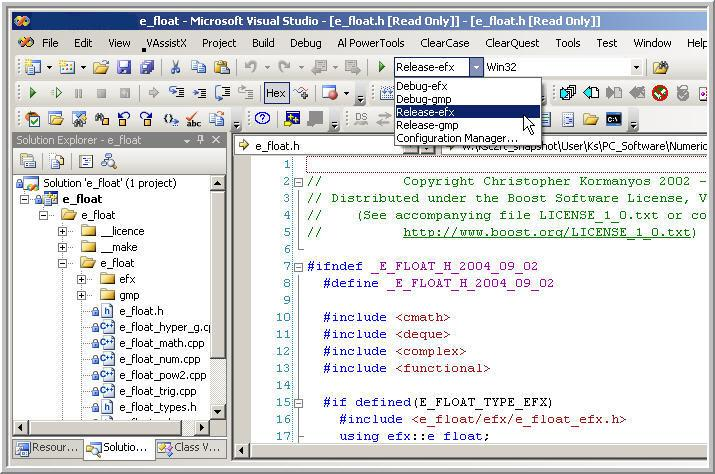
\includegraphics[width=16.0cm]{ef_man_Graphic_200_DevStudioConfig.jpg}
\vspace{0.4cm}
\caption{The \efloat\ configuration selection with Microsoft{\footnotesize {\textregistered}}
Visual Studio{\footnotesize {\textregistered}} 2008 Professional ($+$SP1) is shown. The
project configurations listed in Table \ref{table:systemconfigs} can be selected and built.}
\label{fig:devstudioconfig}
\end{figure}

\noindent \efloat\ can be built within a Windows{\footnotesize {\textregistered}} environment
using Microsoft{\footnotesize {\textregistered}} Visual Studio{\footnotesize {\textregistered}}
2008 Professional with Service Pack $1$ (SP$1$), as shown in Figure~\ref{fig:devstudioconfig}.

\subsubsection{Building the Configurations `efx', `gmp', `mpfr' and `f90' in Windows{\footnotesize {\textregistered}}}

\begin{itemize}
\item Open the solution workspace file
{\courier e\underline\ float/e\underline\ float.sln},
as shown in Figure \ref{fig:devstudioconfig}.
\item Select the appropriate project configuration such as
``release--mpfr'', as shown in Figure \ref{fig:devstudioconfig}
(see Table \ref{table:systemconfigs}).
\item Select 32--bit or 64--bit targets by selecting either ``Win32'' or ``x64'' using
the ``Solution Platforms'' manager.
\item Build the solution with the menu item {\courier Build}$\dots${\courier Build Solution},
or use the corresponding build button.
\item Rebuild the solution with the menu item {\courier Build}$\dots${\courier Rebuild Solution},
or use the corresponding rebuild button.
\item The configurations {\courier gmp} and {\courier mpfr} require GNU~MP and GNU~MP~$+$~MPFR,
respectively. Therefore, GNU MP and MPFR have been ported to
Microsoft{\footnotesize {\textregistered}} Visual Studio{\footnotesize {\textregistered}} 2008
and built for the Windows{\footnotesize {\textregistered}} environment,
based in part on the original porting work provided by
Gladman \cite{gladman:ports}. Separate builds are provided for the 32--bit
Intel{\footnotesize {\textregistered}}
IA32 architecture as well as the 64--bit
Intel{\footnotesize {\textregistered}} Core\ensuremath{^{\text{\courier TM}}}2
architecture (x64). The pre\-built libraries {\courier gmp}.{\courier lib} and {\courier mpfr}.{\courier lib}
for both IA32 as well as x64 have been copied to the respective directories
{\courier p4} and {\courier x64}, which  are subdirectories of the directory
{\courier e\underline\ float/gmp/4-2-4/vc9}. The link commands are already
present within the project file.
\item The configuration {\courier f90} requires the Fortran $90$ wrapper as well as the
corresponding Fortran run--time libraries to be linked with the project.
The Fortran $90$ wrapper {\courier libf90quad}.{\courier lib} has been prebuilt
for both IA32 as well as for x64 using the Intel{\footnotesize {\textregistered}}
Fortran compiler. In addition, the Fortran run--time libraries have been extracted from the
Intel{\footnotesize {\textregistered}} Fortran installation directories for both
IA32 as well as x64.
All of these libraries are stored in the respective directories
{\courier p4} and {\courier x64}, which  are subdirectories of
{\courier e\underline\ float/}{\courier f90/libf90quad/vc9}.
The necessary link commands are already present within the
Microsoft{\footnotesize {\textregistered}} Visual Studio{\footnotesize {\textregistered}}
project file.
\end{itemize}


\subsubsection{Building the Configuration `clr' in Windows{\footnotesize {\textregistered}}}

\begin{itemize}
\item Open the solution workspace file
{\courier e\underline\ float/e\underline\ float.sln},
\item Select the project configuration ``release--clr''.
\item Build the solution with the menu item {\courier Build}$\dots${\courier Build Solution},
or use the corresponding build button.
\item Rebuild the solution with the menu item {\courier Build}$\dots${\courier Rebuild Solution},
or use the corresponding rebuild button.
\item This build configuration produces a
Microsoft{\footnotesize {\textregistered}} Windows{\footnotesize {\textregistered}}~.NET
assembly which can be used with any .NET language in the
Microsoft{\footnotesize {\textregistered}}~CLR.
\end{itemize}

\subsubsection{Building the Configuration `pyd' in Windows{\footnotesize {\textregistered}}}

\begin{itemize}
\item Open the solution workspace file
{\courier e\underline\ float/e\underline\ float.sln},
\item Select the project configuration ``release--pyd''.
\item Build and rebuild the solution as described above.
\item This configuration is only available for the Win32 platform.
\end{itemize}

\subsubsection{Building the Configuration `cas' in Windows{\footnotesize {\textregistered}}}

\begin{itemize}
\item This configuration depends strongly on the selected computer algebra system.
\item An example in given for Mathematica{\footnotesize {\textregistered}}~7.1
for the Win32 platform.
\item Contact the author for detailed instructions when interfacing with
a computer algebra system.
\end{itemize}

\subsection{UNIX--like Environment}

\efloat\ can be built within a UNIX--like environment, such as native UNIX,
native Linux, mingw or cygwin. Building \efloat\ within a UNIX--like
environment requires GCC version $4$.$3$.$1$ or higher
and GNUmake version $3$.$81$ or higher.
In order to successfully build \efloat\ with GCC, it must be verified that
both the version of GCC as well as the version of GNU make are high enough.
These checks can be done by querying the version of GCC (or g$++$) and the
version of GNUmake as shown below.

\vspace{6.0pt}

\lstsetBash
\begin{lstlisting}
chris@desktop:~$ g++ --version
g++ (GCC) 4.3.3
Copyright (C) 2008 Free Software Foundation, Inc.
...
\end{lstlisting}

\vspace{6.0pt}

\lstsetBash
\begin{lstlisting}
chris@desktop:~$ make --version
GNU make 3.81
Copyright (C) 2006 Free Software Foundation, Inc.
...
\end{lstlisting}

\subsubsection{Building the Configurations `efx', `gmp' and `mpfr' in UNIX}

\begin{itemize}
\item For UNIX--like operating systems, \efloat\ can be built using either of the
three MP implementations, {\courier efx}, {\courier gmp} or {\courier mpfr}.
\item The makefile is designed to accept the selection of the {\courier MP} type as an
input parameter, using either {\courier MP$=$efx} or {\courier MP$=$gmp}.
If the {\courier MP} flag is not provided, the default behavior is to build
with {\courier MP$=$efx}.
\item After entering the make command ({\it i.e.} starting the build), the build of the
project should begin and run successfully to completion.
\item The {\courier gmp} build configuration of \efloat\ requires an installed version of GNU MP
because it links with {\courier libgmp.lib} from the GNU MP ({\it i.e.} uses the
link command line switch $-${\courier lgmp}).
\item The {\courier mpfr} build configuration of \efloat\ requires installed versions of GNU~MP
as well as GNU~MP~$+$~MPFR because it links with {\courier libgmp.lib} and {\courier libmpfr.lib} 
({\it i.e.} uses the link command line switches $-${\courier lgmp} $-${\courier lmpfr}).
\end{itemize}

\noindent A sample build command line using {\courier efx::e\underline\ float} is shown in
the command line sequence of the sample bash session below.

\vspace{6.0pt}

\lstsetBash
\begin{lstlisting}
chris@desktop:~$ cd e_float
chris@desktop:~$ make MP=efx
\end{lstlisting}

\noindent A sample build command line using {\courier gmp::e\underline\ float} is shown in
the command line sequence of the sample bash session below.

\vspace{6.0pt}

\lstsetBash
\begin{lstlisting}
chris@desktop:~$ cd e_float
chris@desktop:~$ make MP=gmp
\end{lstlisting}

\noindent The {\courier clean} option of the \efloat\ build is also supported.
Be sure to use the correct value of the build flag {\courier MP} for clean
operations because the clean only cleans intermediate build results of the
selected build configuration. A sample build command line for cleaning the
project with the configuration {\courier gmp} is shown in the bash command
line sequence below.

\vspace{6.0pt}

\lstsetBash
\begin{lstlisting}
chris@desktop:~$ cd e_float
chris@desktop:~$ make clean MP=gmp
\end{lstlisting}


\subsubsection{Building the Configuration `clr' in UNIX}

The {\courier clr} configuration is not currently supported in UNIX.

\subsubsection{Building the Configuration `pyd' in UNIX}

\begin{itemize}
\item Build, rebuild and clean the solution using {\courier{make}}
with the make option {\courier{MP=pyd}}. A dynamic library is built.
\item This build links with the boost python library and the python library
as shown in the makefile. Ensure that these libraries
are properly installed for this build.
\end{itemize}

\subsubsection{Building the Configuration `cas' in Windows{\footnotesize {\textregistered}}}

The {\courier cas} configuration is not currently supported in UNIX.
Specialized support must be developed for the desired computer algebra system.



\pagebreak

\section   {Using \efloathyperref}                   \label{sec:using}
                                                     Using and adapting the \efloat\ system is intuitive and straightforward.
Simple operations used for testing and benchmarking the \efloat\
library can be carried out by modifying the test file {\courier test.cpp}
and rebuilding \efloat, as described in Section \ref{sec:build} above.
Integration of \efloat\ in another independent project would, however,
require a separate build.

\subsection{Real--Numbered Arithmetic with \efloathyperref}

Using {\courier e\underline\ float} objects while coding is natural and
intuitive because {\courier e\underline\ float} objects can be used in
the same way as conventional plain--old--data (POD) floating-point data
types are used. Complete compatibility with the usual C++ semantics for
real--numbered arithmetic has been implemented.
There are also some extra utilities designed for standard situations
which commonly arise in numerical programming. For example, there is as a
globally defined digit tolerance called {\courier ef::tol(void)} within
the name\-space `{\courier ef}'. There is also a convenient
{\courier e\underline\ float} class member function called {\courier order},
which returns the base--$10$ `{big--O}' order of an
{\courier e\underline\ float} object.

The interface to real--numbered arithmetic with \efloat\ objects
is defined in the C++ header file
{\courier <e\underline\ float/e\underline\ float.h>}.
Real valued functions are defined within the name\-space `{\courier ef}'.
A complete synopsis of the \efloat\ class syntax is shown
in Chapter~\ref{chapter:classarch}.
There is no real valued arithmetic interface to any language other than C++.
There is no real valued arithmetic interface to the C language.
The code chunk below illustrates an example of non-trivial,
real valued arithmetic with \efloat\ by showing a possible implementation
of the small-argument Taylor series expansion of $\sin(x)$, $x\in\mathbb{R}$.
Common arithmetic operations and usage of some of the utility functions
are displayed.

\vspace{4.0pt}

\lstsetCPlusPlus
\lstinputlisting{CodeSample_ArithmeticReal.cpp}

\vspace{4.0pt}

The number of decimal digits is fixed at compile--time. The precision can be
dynamically changed during run--time for intermediate calculation steps,
but never increased to more than the fixed number of digits. The
number of digits is set by setting the value of
the preprocessor symbol {\courier E\underline\ FLOAT \underline\ DIGITS10}
which is used to initialize the value of
{\courier ef\underline\ \-digits10\underline\ \-setting},
which is a static constant 32-bit signed integer defined in the
public interface of \efloatbaseclass.

A specialization of the template class
{\courier std::\-nu\-me\-ric\underline\ lim\-its<e\underline\ float>}
has been defined using the usual semantics. This means that it is possible to
query details such as the number of decimal digits of precision or the
maximum \efloatclass\ value in the `usual' manner for the C++ language.
Support for formatted string output using {\courier std::o\-stream}
objects is defined using the usual semantics.
The output stream must be appropriately set
in order to display full precision. A code sample showing numeric limits,
setting output stream precision and printing to output stream is shown below.

\vspace{4.0pt}

\lstsetCPlusPlus
\lstinputlisting{CodeSample_OutputPrecision.cpp}

\vspace{4.0pt}

\subsection{Mixed--Mode Arithmetic with \efloathyperref}

All single--argument \efloatclass\ class constructors have been declared
with the {\courier explicit} qualifier. This prevents unwanted
side--effects such as the automatic compile--time conversion between
POD types and \efloatclass\ objects.
If, for example, the single--argument \efloatclass\ class constructor for
{\courier double} were non--explicit, then this

\vspace{4.0pt}

\lstsetCPlusPlus
\lstinputlisting{CodeSample_ArithmeticAmbiguousCtor.cpp}

\vspace{4.0pt}

\noindent would be ambiguous because the compiler would use conventional
double--precision for the sin function and subsequently convert to
an \efloatclass\ result. This would compromise the precision of the final
result because one of its intermediate calculation values would only have
the precision of {\courier double}.

However, even though all constructors \efloatclass\ class constructors
from POD types are explicit, there is support for global operators
for multiplication and division with constant {\courier INT32}.
These operations are exact and non--ambiguous because the representation
of {\courier INT32} is exact and non--ambiguous. Using the global
{\courier INT32} multiplication operator is shown in the code sample below.

\vspace{4.0pt}

\lstsetCPlusPlus
\lstinputlisting{CodeSample_ArithmeticMixedMode.cpp}

\vspace{4.0pt}

\noindent Remarking further on the code sample above, some users might expect
\efloatclass\ class constructors from integer types to be non--explicit
because the representation of integer types is exact and non--ambiguous.
However, the \efloatclass\ class constructors from integer types are
nonetheless declared explicit. Otherwise some common C++ code sequences would
lead to non--intuitive, confusing results. For example, this sequence

\vspace{4.0pt}

\lstsetCPlusPlus
\lstinputlisting{CodeSample_ArithmeticConfusingIfNonexplicitIntCtor.cpp}

\vspace{4.0pt}

\noindent might be expected to produce the value of $\frac{1}{7}$ to full precision.
This might be expected from the perspective of a symbolic system such as a
computer algebra system. But in fact, the C++ compiler actually reduces the value
of $\frac{1}{7}$ to $0$ in this case. The subsequent C++ initialization is
carried out with the pure--integer value $0$ instead of the full decimal
value of $\frac{1}{7}$. This situation is somewhat non--intuitive and confusing.
In order to facilitate non--ambiguity in these kinds of situations and to
avoid unexpected compiler side--efects, all \efloatclass\ constructors
from integer types are declared {\courier explicit}. Therefore when writing
code for these kinds of situations, the proper way to initialize fractions
such as $\frac{1}{7}$ or $\frac{1}{12}$ is like this

\vspace{4.0pt}

\lstsetCPlusPlus
\lstinputlisting{CodeSample_ArithmeticInitOneSeventh.cpp}

\vspace{4.0pt}

\noindent The strict use of the C++ style static cast could
be considered optional from a stylistic point of view.
Nonetheless, the author prefers to include the static cast
because this improves code portability by reducing
the degrees of freedom which exist for compiler interpretation
of the plain integer data type.


\subsection{Complex--Numbered Arithmetic with \efloathyperref}

Complex valued arithmetic is supported with the class {\courier ef\underline\ complex},
which has the same public interface as the STL template class
{\courier std::complex<{\it typename T}>}.
Complex valued functions are defined within the name\-space `{\courier efz}'.
The interface to complex valued arithmetic with {\courier ef\underline\ complex}
objects is defined in the C++ header file
{\courier <e\underline\ float/e\underline\ float\underline\ z.h>}.
Complex {\ttfamily ef\underline\ complex} objects can be used with each other
in normal arithmetic expressions and also mixed together with real
{\courier e\underline\ float} objects.
There is no complex valued arithmetic interface to any language other than C++.
There is no complex valued arithmetic interface to the C language.
The following code snippet displays the basic
use of {\ttfamily ef\underline\ complex} objects.

\vspace{4.0pt}

\lstsetCPlusPlus
\lstinputlisting{CodeSample_ArithmeticComplex.cpp}

\vspace{4.0pt}

\subsection{Using the \efloathyperref\ Functions}

\vspace{3.0pt}

Using the \efloat\ library of functions is straightforward. All of the
function prototypes are declared in C++ header files.
These have been collected in a single header file called
{\courier <func\-tions/\-func\-tions.h>} which contains
both real valued functions as well as complex valued
functions. The function prototypes are C++ function prototypes written in the
C++ language. There is no functional interface to any language other than C++.
There is no functional interface to the C language. A complete listing of the
functions supported by \efloat\ is provided in Section \ref{sec:functions}.
A use of functions is shown in the code snippet below.

\vspace{4.0pt}

\lstsetCPlusPlus
\lstinputlisting{CodeSample_Functions.cpp}

\vspace{4.0pt}

\subsection{Using the STL with \efloathyperref\ objects}

Real \efloat\ objects and complex
{\courier ef\underline\ complex} objects can be used
without limitation in standard STL containers and algorithms.
Both \efloat\ and {\courier ef\underline\ complex}
objects as well as pointers to these objects can be stored in all standard
STL and TR1 containers such as STL's template
{\courier std::\-vec\-tor<{\it typename T}>} class or TR1's template
{\courier std::\-tr1::\-array<{\it typename T}, {\courier std::\-size\underline\ t} {\it N}>}
class. This provides for powerful manipulation with STL algorithms such as
sorting, accumulating, streaming to output streams, etc. A use of
\efloat\ with a container, an algorithm, iterators, and stream output
is shown in the code sample below.

\vspace{4.0pt}

\lstsetCPlusPlus
\lstinputlisting{CodeSample_STL_Use.cpp}

\vspace{4.0pt}

\subsection{Additional Examples Using \efloathyperref}

Additional practical applications of \efloat\ are provided by seven
hand--written example files. The example files are stored in
{\courier{examples/example}}$\ast${\courier{.cpp}}, and they are
part of the tools block.

Example $1$ shows real--numbered usage in combination
with a timing measurement. It calculates $21$ non--trivial
values of $P_{\nu}^{\mu}(x)$, with $\nu$,$\,\mu$,$\,x\in\mathbb{R}$.
Example $2$ shows complex--num\-ber\-ed usage in combination
with a timing measurement. It calculates $21$ non--trivial
values of $\zeta(s)$, with $s\in\mathbb{Z}$.

Example $3$ shows mixed mode, real/integer operation by calculating the
real--num\-ber\-ed Jahnke--Emden--Lambda function,
$\Lambda_{\nu}(x)=\left\{\Gamma(\nu+1)\,J_{\nu}(x)\right\}\,/\,\left(\frac{1}{2}x\right)^{\nu}$
\cite{jahnkeemden:textbook}.
The small--argument series expansion employs arithmetic
operations as well as mixed--mode calculations.
It also shows how to effectively use STL containers of
{\courier{e{\ttfamily\underline\ }float}}
objects with STL algorithms.

Examples $4$ and $5$ use template utilities from the tools block.
Example $4$ performs a numerical differentiation,
$\frac{\partial}{\partial\nu}\,J_{\nu}(151+\gamma)\big|_{(\nu=123+C)}\,$,
where $\gamma$ is Euler's constant and $C$ is Catalan's constant.
The derivative central difference rule is ill--conditioned
and does not maintain full precision.
Example $5$ calculates a numerical integral,
$J_{0}(x)=\frac{1}{\pi}\int_{0}^{\pi}\,\cos(x\,\sin t)\,dt$, with $x=\left(12+\gamma\right)$
using a recursive trapezoid rule.
The utilities in Examples 4 and 5 make use of advanced
object--oriented templates. These examples show how static and dynamic
polymorphism can be combined to make efficient, elegant implementations
for standard numerical tasks.

In example~$6$, some well--known conventional algorithms are extended
to high precision and redesigned for use with real as well as complex
numbers. Luke~\cite{lukealgo:textbook} developed quadruple--precision
algorithms in For\-tran~$77$ which calculate coefficients for expansions
of hy\-per\-ge\-o\-me\-tric functions in series of Cheb\-y\-shev polynomials.
Luke's algorithms
{\courier{CCOEF2}} for $_{2}F_{1}(a, b; c; z)$ on page 59,
{\courier{CCOEF3}} for $_{1}F_{1}(a; b; z)$ on page 74,
and
{\courier{CCOEF6}} for $_{1}F_{2}(a; b, c; z)$ on page 85
have been extended to high precision. The inner loops have been
simplified through analyses with a computer algebra system.
Furthermore, these algorithms have been implemented as templates
for simultaneous use with real as well as complex pa\-ra\-me\-ters.
Table~\ref{table:functions} shows that \efloat's implementations
of hy\-per\-ge\-o\-me\-tric functions have strong limitations on their
parameter ranges. Example $6$ takes a promising first step toward
extending these parameter ranges.

Example~$7$ shows \efloat's interoperability with
the Math\-Link{\footnotesize {\textregistered}} facility of \mathematica.
Template programs combined with \efloat's
interface to computer algebra systems are used to
implement the generalized complex poly\-gam\-ma function
$\psi_{\nu}(x)$, with $\nu$,$\,x\in\mathbb{R}$ or $\mathbb{Z}$.
This extends the functionality of \efloat\ since its native al\-go\-rithm,
$\psi_{n}(x)$, only supports real parameters.

\subsection{Interoperability In Detail}

\subsubsection{Python~Export}
The \efloat\ export to Python produces a dynamic,
shared library. It is called
``{\courier{e{\ttfamily\underline\ }float{\ttfamily\underline\ }pyd.}}$\ast$'',
where the file ending will be either ``{\courier{pyd}}''
or ``{\courier{so}}'' for Windows{\footnotesize {\textregistered}} or
Unix/Linux--GNU systems respectively.
The shared library can be loaded into Python and the functions and classes of
\efloat\ can be used with its high level scripting capabilities
such as list manipulation. Interoperability with
mpmath~\cite{mpmath:website} can be achieved with Python strings.
The Python session below shows how to load the shared library and
generate a list of function values.
The final print command needs two carriage returns.

\lstset{language=python, basicstyle=\courierEight, keywordstyle=\ttfamily}
\begin{lstlisting}
>>> import e_float_pyd
>>> from e_float_pyd import(e_float, ef_complex, ef, efz)
>>> lst=[ef.cyl_bessel_j(ef.third(), k + ef.quarter()) for k in range(10)]
>>> for y in lst: print y
\end{lstlisting}

\subsubsection{Microsoft{\footnotesize {\textregistered}}~CLR~Export}
The \efloat\ export to the Microsoft{\footnotesize {\textregistered}} CLR
creates a CLR assembly for the Microsoft{\footnotesize {\textregistered}}.net Framework.
The name of the assembly is 
``{\courier{e{\ttfamily\underline\ }float{\ttfamily\underline\ }clr}}.{\courier{dll}}''.
It can be used with
all Microsoft{\footnotesize {\textregistered}} CLR
languages including C\#, managed C++/CLI, IronPython, {\emph{etc}}.
The code below illustrates the syntax of \efloat\ in the C\# language.

\lstset{language=[ISO]C++,basicstyle=\courierEight,commentstyle=\itshape,
keywordstyle=\bfseries,extendedchars=true}
\begin{lstlisting}
using e_float_clr.cli;
namespace test
{
  class Program
  {
    static void Main(string[] args)
    {
      e_float x = ef.half();
      e_float y = new e_float(123);
      ef_complex z = efz.riemann_zeta(new ef_complex(x, y));

      System.Console.WriteLine(z.get_str());
    }
  }
}
\end{lstlisting}


\subsubsection{Computer Algebra Systems}
Using a computer algebra system from within \efloat, in particular
extending \efloat\ with \mathematica, has
been discussed previously in Example~7.
The architecture for this is in the directory
{\courier{interop/cas}}. It uses an abstract base class called
{\courier{Com\-pu\-ter\-Al\-ge\-bra\-Sys\-tem\-Ob\-ject}} whose public interface
defines generic methods which exchange information with a
computer algebra system using STL strings and containers of \efloatclass\ objects.
The other interoperability direction,
using \efloat\ from within \mathematica, is not yet supported.


\pagebreak

\section   {The \efloathyperref\ Class Architecture} \label{chapter:classarch}
                                                     The class architecture of the \efloat\ system has been described in
Section~\ref{sec:architecture}. The architecture is based on three main
components: the \efloatbaseclass\ class, the \efloatclass\ class and the
\efloatclass\ global arithmetic interface. The synopsis of these components is
described in the following sections.

\subsection{The \efloatbasehyperref\ Class}\label{subsec:efbaseclass}

The \efloatbaseclass\ class is a partly abstract base class from which the
\efloatclass\ class is derived. The $33$ public pure--virtual interface functions
of the \efloatbaseclass\ class describe all mathematical primitives needed
for real--numbered arithmetic.
The synopsis of the public interface to the \efloatbaseclass\ class is shown below.

\vspace{4.0pt}

\lstsetCPlusPlus
\lstinputlisting{CodeSample_EfloatBaseSynopsis.cpp}

\vspace{4.0pt}

\subsection{The \efloathyperref\ Class}\label{subsec:efclass}

The \efloatclass\ class implements all of the pure--virtual functions
of its base class and adds additional numerical constants and local
private utility functions.
The synopsis of the public interface to the \efloatclass\ class is shown below.

\vspace{4.0pt}

\lstsetCPlusPlus
\lstinputlisting{CodeSample_EfloatSynopsis.cpp}

\vspace{4.0pt}

\subsection{The \efloathyperref\ Global Arithmetic Interface}

The \efloatclass\ global arithmetic interface defines global functions
for arithmetic.
The synopsis of the \efloatclass\ global arithmetic interface is shown below.

\vspace{4.0pt}

\lstsetCPlusPlus
\lstinputlisting{CodeSample_EfloatGlobalMathSynopsis.cpp}

\vspace{4.0pt}

\subsection{Numeric Limits of the \efloathyperref\ Class}

In order to maintain consistency with C++ programming styles and idioms,
a template specialization of STL's standard numeric limits class has
been implemented. It is called
{\courier std::\-nu\-me\-ric\underline\ lim\-its<e\underline\ float>}.
The class synopsis is shown below.

\vspace{4.0pt}

\lstsetCPlusPlus
\lstinputlisting{CodeSample_EfloatNumLimSynopsis.cpp}

\vspace{4.0pt}

\subsection{Adapting Another MP Implementation for use with \efloathyperref}

From a software--architectural standpoint, it is quite straightforward
to adapt another MP implementation for use with \efloat.
In order to be used with \efloat, the MP needs to be implemented in a
class which is called \efloatclass. This adapted MP class must be
derived from the \efloatbaseclass\ class and it must also reside
within a unique namespace. Furthermore, the adapted MP class must fully
implement all of the $33$ pure--virtual functions of \efloatbaseclass,
which are listed in Section~\ref{subsec:efbaseclass}.
Although architecturally simple enough, the actual implementation details
of the functions needed for the
virtual interface --- such as fast multiplication --- can be
technically very challenging to implement in an efficient fashion.

Any optional number of the virtual functions needed for
the ``{\emph has--its--own}'' mechanism should also be implemented such
that they return {\courier true} if the MP's own function should
be used. Be sure to also implement the corresponding static functions.

When the adapted MP type is fully implemented, it can be selected
with a compile--time definition and used as a drop--in replacement
for the selected MP type in \efloat.

\subsection{The Complex Class Interface}

The \efcomplexclass\ class defines the \efloat\ interface to
complex--numbered values. The synopsis of the public interface
to the \efcomplexclass\ class is shown below.

\vspace{4.0pt}

\lstsetCPlusPlus
\lstinputlisting{CodeSample_EfloatComplexSynopsis.cpp}

\vspace{4.0pt}



\pagebreak

\section   {The \efloathyperref\ Functions}          \label{sec:functions}
                                                     \subsection{Supported Functions and Known Limitations}


\begin{table}[p]\noindent
\begin{center}
\renewcommand{\arraystretch}{1.00}
\begin{tabular}{l|l|l|l}

Symbol
             & Name
             & Parameters
             & Known Limitations \\

\hline

$+$, $-$, $\times$, $\div$, $=$, {\it etc}
             & operations
             & $x,y \in \mathbb{R}$; $x,y \in \mathbb{Z}$
             & \ \\

$+$$=$, $-$$=$, $\times$$=$, $\div$$=$, {\it etc}
             & self--operations
             & $x,y \in \mathbb{R}$; $x,y \in \mathbb{Z}$
             & \ \\

$<$, $\leq$, $>$, $\geq$, $==$, $!$$=$
             & comparisons
             & $x,y \in \mathbb{R}$
             & \ \\

$x\rightarrow$ {\courierNine INT64}, {\courierNine double}, {\it etc}
             & convert $\mathbb{R}$
             & $x \in \mathbb{R}$
             & \ \\

$x\rightarrow$ {\courierNine std::complex<double>}
             & convert $\mathbb{Z}$
             & $x \in \mathbb{Z}$
             & \ \\

$x\rightarrow$ {\courierNine std::string}, {\it etc}
             & convert {\courier char}
             & $x \in \mathbb{R}$;  $x \in \mathbb{Z}$
             & \ \\

{\courierNine std::ostream\ <{}<{}}$\,x$
             & output stream
             & $x \in \mathbb{R}$;  $x \in \mathbb{Z}$
             & \ \\

fabs$(x)$, floor$(x)$, {\it etc}
             & math convert
             & $x,y \in \mathbb{R}$
             & \ \\

$x_{{\mbox{{\courierSeven{frac}}}}}$, $x_{{\mbox{{\courierSeven{int}}}}}$
             & constituents
             & $x \in \mathbb{R}$
             & \ \\

1, 2, $\frac{1}{3}$, {\courier INT32$_{{\mbox{{\courierSeven{max}}}}}$}, {\it etc}
             & rationals
             & $\in \mathbb{Q}$
             & \ \\

$\sqrt{2}$, $\pi$, $e$, $\log(2)$, $\gamma$, {\it etc}
             & constants
             & $\in \mathbb{R}$, $\notin \mathbb{Q}$
             & \ \\

$n!$, $n!!$, $B_{n}$, $E_{n}$, {\it etc}
             & int functions
             & $n \in \mathbb{N}^{+}$
             & $n \lesssim 10^{6}$ \\

$P_{n}$
             & primes
             & $n \in \mathbb{N}^{+}$
             & $n \lesssim 10^{6}$ \\

$n=\prod P_{i}$
             & prime factors
             & $n \in \mathbb{N}^{+}$
             & $n \lesssim 10^{9}$ \\

$e^x$, $x^a$
             & power
             & $x, a \in \mathbb{R}$; $x, a \in \mathbb{Z}$
             & \ \\

$\log(x), \log_{a}(x)$
             & logarithmic
             & $x, a \in \mathbb{R}$; $x, a \in \mathbb{Z}$
             & \ \\

$\sin(x)$, $\cos(x)$, {\it etc}
             & trigonometric
             & $x \in \mathbb{R}$; $x \in \mathbb{Z}$
             & $\left|\Re(x)\right| \lesssim 10^{20}$ \\

asin$(x)$, acos$(x)$, {\it etc}
             & \ %space
             & $x \in \mathbb{R}$; $x \in \mathbb{Z}$
             & \ \\

$\sinh(x)$, $\cosh(x)$, {\it etc}
             & hyperbolic
             & $x \in \mathbb{R}$; $x \in \mathbb{Z}$
             & \ \\

asinh$(x)$, acosh$(x)$, {\it etc}
             & \ %space
             & $x \in \mathbb{R}$; $x \in \mathbb{Z}$
             & \ \\

$Ai(x)$,$\,Bi(x)$,$\,Ai^{\prime}(x)$,$\,Bi^{\prime}(x)$
             & Airy
             & $x \in \mathbb{R}$
             & $-10^{10} \lesssim x \lesssim 10^{4}$ \\

$J_{\nu}(x)$,$\,Y_{\nu}(x)$,$\,K_{\nu}(x)$,$\,I_{\nu}(x)$
             & Bessel
             & $x \in \mathbb{R}$; $\nu \in \mathbb{R}$
             & $\left|\nu\right| \lesssim 10^{9}$ \\

$T_{n}(x)$,$\,U_{n}(x)$,$\,L_{n}(x)$,$\,H_{n}(x)$
             & polynomial
             & $x \in \mathbb{R}$; $x \in \mathbb{Z}$;
             & $\left|n\right| \lesssim 10^{5}$ \\

\ %space
             & \ %space
             & $n \in \mathbb{N}^{+}$
             & \ \\

$\Gamma(x)$, $(x)_{a}$, {\it etc}
             & gamma
             & $x, a \in \mathbb{R}$; $x, a \in \mathbb{Z}$
             & \ \\

$\Gamma(x, a)$
             & incomp gamma
             & $x, a \in \mathbb{R}$
             & $\left|a\right| \lesssim 10^{2}$ \\

$\psi^{n}(x)$
             & poly\-gamma
             & $x \in \mathbb{R}$; $n \in \mathbb{N}^{+}$,
             & $0 \leq n \lesssim 10^{2}$ for $x < 0$ \\

$_{1}F_{1}(a, b; x)$
             & conf hyperg
             & $x \in \mathbb{R}$
             & $\left|a\right|$,$\,\left|b\right| \lesssim 10^{2}$ \\

$_{p}F_{q}(a_{1},\dots a_{p}; b_{1},\dots b_{q}; x)$
             & hyperg
             & $x \in \mathbb{R}$; $p,q \in \mathbb{N}^{+}$;
             & $\left|x\right| \leq 1$; only partial \\

\ %space
             & \ %space
             & $a_{n}, b_{n} \in \mathbb{R}$;
             & support for $a_{n} \in \mathbb{N}^{-}$; \\

\ %space
             & \ %space
             & \ %space
             & $\left|a\right|$,$\,\left|b\right| \lesssim 10$ \\

$P_{\nu}^{\mu}(x)$, $Q_{\nu}^{\mu}(x)$
             & Legendre
             & $x \in \mathbb{R}$; $\nu,\mu \in \mathbb{R}$
             & $\left|x\right| \leq 1$; $\left|\nu\right|$,$\,\left|\mu\right| \lesssim 10^{5}$; \\

\ %space
             & \ %space
             & \ %space
             & $Q_{\nu}^{\mu}(x)$ could be NaN if \\

\ %space
             & \ %space
             & \ %space
             & $\nu$, $\mu \ni\mathbb{N}$, but $\nu$$\,+\,$$\mu\in\mathbb{N}$ \\

$L_{\nu}^{\lambda}(x)$
             & Laguerre
             & $x \in \mathbb{R}$; $\nu,\lambda \in \mathbb{R}$
             & $\left|\nu\right|$,$\,\left|\lambda\right| \lesssim 10^{2}$ \\

$D_{\nu}(x)$
             & parabolic cyl
             & $x \in \mathbb{R}$; $\nu \in \mathbb{R}$
             & $\left|\nu\right| \lesssim 10^{5}$ \\

$H_{\nu}(x)$
             & Hermite
             & $x \in \mathbb{R}$; $\nu \in \mathbb{R}$
             & $\left|\nu\right| \lesssim 10^{5}$ \\

$E(\phi, m)$, $F(\phi, m)$, $K(m)$
             & Elliptic
             & $\phi, m \in \mathbb{R}$
             & $0 \leq m \leq 1$ \\

$\zeta(s)$
             & Riemann zeta
             & $s \in \mathbb{R}$; $s \in \mathbb{Z}$
             & $\left|\Im(s)\right| \lesssim 10^{6}$ \\

$\zeta(s, a)$
             & Hurwitz zeta
             & $s, a \in \mathbb{R}$; $s, a \in \mathbb{Z}$
             & $\left|\Im(s)\right| \lesssim 10^{6}$; \\

\ %space
             & \ %space
             & \ %space
             & $\Re(s) \gtrsim -10$ \\

Li$_n(x)$
             & poly\-log
             & $x \in \mathbb{R}$; $x \leq 1$;
             & $n \in \mathbb{N}^{+}$ for $x < 0$ \\

\ %space
             & \ %space
             & $n \in \mathbb{N}$
             & \ \\
\hline
\end{tabular}
\vspace{2.0mm}
\caption{The functions supported by \efloat, including their parameters
and known limitations (other than overflow and underflow), are listed.}
\label{table:functions}
\end{center}
\end{table}


The functions supported by \efloat\ including parameter ranges and
known limitations are listed in Table~\ref{table:functions}.
There is support for many functions and also
for wide ranges of function parameters.
Several functions such as Bessel functions and Legendre functions
include very large parameter ranges, unavailable from other systems.
The \efloat\ system has been designed for $30$ to $300$ decimal digits of precision.
Complex arithmetic is supported and elementary
functions are implemented for real and complex numbers.
The special functions are implemented primarily for real parameters,
but some also accept complex parameters.

\pagebreak

\subsection{Function Details}

The following sections briefly describe the functions which are implemented in
the \efloat\ library. Only very terse mathematical descriptions of the functions
are provided, for example the primary function definition or a single series
expansion at one point such as zero or one. The brief descriptions and
remarks are only meant to uniquely define the functions and do not provide
complete descriptions of the algorithms and computations. The actual calculations
in the \efloat\ library use many additional algorithms and function representations,
often involving hyper\-geometric series or precomputed tables, to calculate function
values over wide parameter ranges. Real valued functions are defined
within the name\-space `{\courier ef}'. Utility functions are defined
within the name\-space `{\courier ef}'. Complex valued functions are defined
within the name\-space `{\courier efz}'.

\subsubsection{Integer and Constant Functions} \lstsetCPlusPlus
\begin{lstlisting}
const e_float& zero         (void);
const e_float& one          (void);
const e_float& two          (void);
const e_float& three        (void);
const e_float& four         (void);
const e_float& five         (void);
const e_float& six          (void);
const e_float& seven        (void);
const e_float& eight        (void);
const e_float& nine         (void);
const e_float& ten          (void);
const e_float& twenty       (void);
const e_float& thirty       (void);
const e_float& forty        (void);
const e_float& fifty        (void);
const e_float& hundred      (void);
const e_float& two_hundred  (void);
const e_float& three_hundred(void);
const e_float& four_hundred (void);
const e_float& five_hundred (void);
const e_float& thousand     (void);
const e_float& two_k        (void);
const e_float& three_k      (void);
const e_float& four_k       (void);
const e_float& five_k       (void);
const e_float& ten_k        (void);
const e_float& twenty_k     (void);
const e_float& thirty_k     (void);
const e_float& forty_k      (void);
const e_float& fifty_k      (void);
const e_float& hundred_k    (void);
const e_float& million      (void);
const e_float& ten_M        (void);
const e_float& hundred_M    (void);
const e_float& billion      (void);
const e_float& int32max     (void);
const e_float& int32min     (void);
const e_float& int64max     (void);
const e_float& int64min     (void);
const e_float& one_minus    (void);
const e_float& tenth        (void);
const e_float& fifth        (void);
const e_float& quarter      (void);
const e_float& third        (void);
const e_float& half         (void);
const e_float& two_third    (void);
const e_float& four_third   (void);
const e_float& three_half   (void);
\end{lstlisting}

\vspace{6.0pt}

\noindent {\it Returns:} These functions return a static constant
reference to the precomputed value of the respective rational number.

\lstsetCPlusPlus
\begin{lstlisting}
const e_float& sqrt2        (void);
const e_float& sqrt3        (void);
const e_float& pi           (void);
const e_float& pi_half      (void);
const e_float& pi_quarter   (void);
const e_float& pi_squared   (void);
const e_float& two_pi       (void);
const e_float& sqrt_pi      (void);
const e_float& degree       (void);
const e_float& exp1         (void);
const e_float& ln2          (void);
const e_float& ln3          (void);
const e_float& ln10         (void);
const e_float& log10_2      (void);
const e_float& golden_ratio (void);
const e_float& euler_gamma  (void);
const e_float& catalan      (void);
const e_float& khinchin     (void);
const e_float& glaisher     (void);
\end{lstlisting}

\vspace{6.0pt}

\noindent {\it Returns:} These functions return a static constant
reference to the precomputed value of the respective mathematical constant.

\vspace{6.0pt}

\lstsetCPlusPlus
\begin{lstlisting}
void prime(const UINT32 n, std::deque<UINT32>& primes);
\end{lstlisting}

\vspace{6.0pt}

\noindent {\it Effects:} This function calculates the first {\courier n}
prime numbers and stores them in the container {\courier primes}.

\lstsetCPlusPlus
\begin{lstlisting}
void integer_factors(const UINT32 n, std::deque<Util::point_nm>& pf);
\end{lstlisting}

\noindent {\it Effects:} This function calculates the prime
factorization of the unsigned integer {\courier n} and
stores the results as ordered sequence of integer pairs in
the container {\courier pf}.

\vspace{6.0pt}

\noindent {\it Remark:} The functions {\courier prime} and
{\courier integer\underline\ factors} are implemented as utility functions.
They are not intended for high-performance use.

\vspace{6.0pt}

\lstsetCPlusPlus
\begin{lstlisting}
e_float euler    (const UINT32 n);
e_float bernoulli(const UINT32 n);
e_float stirling2(const UINT32 n, const UINT32 k);
\end{lstlisting}

\noindent {\it Effects:} These functions calculate the integer function
of the respective arguments.

\vspace{6.0pt}

\noindent {\it Returns:} The {\courier euler} function returns the signed integer
number which can be defined by the identity \cite{wiki:website}

\vspace{6.0pt}

\begin{equation}
\frac{1}{\cosh(x)} = \frac{2}{e^{x}+e^{-x}}
\equiv \sum_{n=0}^{\infty} \frac{E_{n}x^{n}}{n!}.
\end{equation}

\noindent {\it Returns:} The {\courier bernoulli} function returns the signed rational
number which can be defined by the identity \cite{wolframfunctions:website}

\vspace{6.0pt}

\begin{equation}
\frac{x}{e^{x}-1}\equiv \sum_{n=0}^{\infty} \frac{B_{n}x^{n}}{n!}.
\end{equation}

\noindent {\it Returns:} The {\courier stirling2} function returns the unsigned integer
Stirling number of the second kind given by the formula \cite{wiki:website}

\vspace{6.0pt}

\begin{equation}
S(n, k) = {\genfrac{\{}{\}}{0pt}{}{n}{k}} = \frac{1}{k!}
\sum_{j=0}^{k}(-1)^{k-j}\binom{k}{j} j^{n}.
\end{equation}


\subsubsection{Elementary Functions}           \lstsetCPlusPlus
\begin{lstlisting}
// Utility functions for real and complex valued arguments.
bool isnan(const double x);
bool isnan(const e_float& x);
bool isnan(const ef_complex& z);

bool finite(const double x);
bool finite(const e_float& x);
bool finite(const ef_complex& z);

bool isneg(const double x);
bool isneg(const e_float& x);
bool isneg(const ef_complex& z);

e_float fabs(const e_float& x);
e_float abs (const e_float& x);
e_float abs (const ef_complex& z);
e_float real(const e_float& x);
e_float real(const ef_complex& z);
e_float imag(const e_float& x);
e_float imag(const ef_complex& z);

bool ispos(const double x);
bool ispos(const e_float& x);
bool ispos(const ef_complex& z);

bool isint(const double x);
bool isint(const e_float& x);
bool isint(const ef_complex& z);

bool isone(const double x);
bool isone(const e_float& x);
bool isone(const ef_complex& z);

bool iszero(const double x);
bool iszero(const e_float& x);
bool iszero(const ef_complex& z);

double to_double(const double& x);
double to_double(const e_float& x);

INT64 to_int64(const double x);
INT64 to_int64(const e_float& x);
INT64 to_int64(const ef_complex& z);

bool small_arg(const double x);
bool small_arg(const e_float& x);
bool small_arg(const ef_complex& z);
\end{lstlisting}

\vspace{6.0pt}

\noindent {\it Returns:} These functions return the given utility function
for their respective arguments.

\vspace{6.0pt}

\noindent {\it Remark:} The real valued {\courier real} function returns its argument
and the real valued {\courier imag} function returns zero.

\vspace{6.0pt}

\noindent {\it Remark:} The functions {\courier isint} and {\courier isone}
test for integer values within a tolerance.

\vspace{6.0pt}

\noindent {\it Remark:} The {\courier small\underline\ arg} function
tests if $|${\courier x}$|$~$\stackrel{?}{\lesssim} 10^{-d/6}$, where
$d$ is the number of decimal digits of precision of the underlying type.

\lstsetCPlusPlus
\begin{lstlisting}
// Elementary real valued functions using the C++ naming convention.
e_float floor     (const e_float& x);
e_float ceil      (const e_float& x);
e_float pow2      (const INT64 p);
e_float pown      (const e_float& x, const INT64 p);
e_float inv       (const e_float& x);
e_float sqrt      (const e_float& x);
e_float sqrt1pm1  (const e_float& x);
e_float cbrt      (const e_float& x);
e_float rootn     (const e_float& x, const INT32 p);
e_float exp       (const e_float& x);
e_float log       (const e_float& x);
e_float log10     (const e_float& x);
e_float loga      (const e_float& x, const e_float& a);
e_float log1p     (const e_float& x);
e_float log101p   (const e_float& x);
e_float loga1p    (const e_float& x, const e_float& a);
e_float log1p1m2  (const e_float& x);
e_float pow       (const e_float& x, const e_float& a);
e_float powm1     (const e_float& x, const e_float& a);
void    sincos    (const e_float& x, e_float* const p_sin,
                                     e_float* const p_cos);
e_float sin       (const e_float& x);
e_float cos       (const e_float& x);
e_float tan       (const e_float& x);
e_float csc       (const e_float& x);
e_float sec       (const e_float& x);
e_float cot       (const e_float& x);
e_float asin      (const e_float& x);
e_float acos      (const e_float& x);
e_float atan      (const e_float& x);
e_float atan2     (const e_float& y, const e_float& x);
void    sinhcosh  (const e_float& x, e_float* const p_sin,
                                     e_float* const p_cos);
e_float sinh      (const e_float& x);
e_float cosh      (const e_float& x);
e_float tanh      (const e_float& x);
e_float asinh     (const e_float& x);
e_float acosh     (const e_float& x);
e_float atanh     (const e_float& x);
\end{lstlisting}

\vspace{6.0pt}

\noindent {\it Returns:} These functions return the real value of the corresponding
elementary function for their respective real valued arguments.

\vspace{6.0pt}

\noindent {\it Remark:} Not every function has a counterpart function in C or C++.

\vspace{6.0pt}

\noindent {\it Remark:} The {\courier sqrt1pm1} function returns $\sqrt{1 + x} - 1$,
for small $x$.

\vspace{6.0pt}

\noindent {\it Remark:} The {\courier log1p} function returns $\log(1 + x)$.
The {\courier log101p} function returns $\log_{10}(1 + x)$.
The {\courier loga1p} function returns $\log_{a}(1 + x)$.

\vspace{6.0pt}

\noindent {\it Remark:} The {\courier log1p1m2} function returns
$(1/2)\log\left[(1+x)/(1-x)\right]$.

\vspace{6.0pt}

\noindent {\it Remark:} The {\courier powm1} function returns $x^{a} - 1$ for
$x$ near one.

\lstsetCPlusPlus
\begin{lstlisting}
// Elementary complex valued functions using the C++ naming convention.
ef_complex polar   (const e_float& mod, const e_float& arg);
ef_complex conj    (const ef_complex& z);
ef_complex iz      (const ef_complex& z);
ef_complex sin     (const ef_complex& z);
ef_complex cos     (const ef_complex& z);
ef_complex tan     (const ef_complex& z);
void       sincos  (const ef_complex& z, ef_complex* const p_sin,
                                         ef_complex* const p_cos);
ef_complex csc     (const ef_complex& z);
ef_complex sec     (const ef_complex& z);
ef_complex cot     (const ef_complex& z);
ef_complex asin    (const ef_complex& z);
ef_complex acos    (const ef_complex& z);
ef_complex atan    (const ef_complex& z);
ef_complex inv     (const ef_complex& z);
ef_complex sqrt    (const ef_complex& z);
ef_complex exp     (const ef_complex& z);
ef_complex log     (const ef_complex& z);
ef_complex log10   (const ef_complex& z);
ef_complex loga    (const ef_complex& z, const ef_complex& a);
ef_complex pown    (const ef_complex& z, const INT64 p);
ef_complex pow     (const ef_complex& z, const ef_complex& a);
ef_complex rootn   (const ef_complex& z, const INT32 p);
ef_complex sinh    (const ef_complex& z);
ef_complex cosh    (const ef_complex& z);
ef_complex tanh    (const ef_complex& z);
void       sinhcosh(const ef_complex& z, ef_complex* const p_sinh,
                                         ef_complex* const p_cosh);
ef_complex asinh   (const ef_complex& z);
ef_complex acosh   (const ef_complex& z);
ef_complex atanh   (const ef_complex& z);
\end{lstlisting}

\vspace{6.0pt}

\noindent {\it Returns:} These functions return the complex value of the corresponding
elementary function for their respective complex valued arguments.

\vspace{6.0pt}

\noindent {\it Remark:} Not every function has a counterpart function in C or C++.


\subsubsection{Airy Functions}                 \lstsetCPlusPlus
\begin{lstlisting}
e_float airy_a      (const e_float& x);
e_float airy_a_prime(const e_float& x);
e_float airy_b      (const e_float& x);
e_float airy_b_prime(const e_float& x);
\end{lstlisting}

\vspace{6.0pt}

\noindent {\it Effects:} These functions compute the Airy functions and derivatives
for their respective argument {\courier x}, with {\courier x}~$\in\mathbb{R}$.

\vspace{6.0pt}

\noindent {\it Returns:} The {\courier airy\underline\ a} function
returns~\cite{wolframfunctions:website}

\begin{equation}
Ai(x) =
\frac{1}{3^{2/3} \Gamma(\frac{2}{3})}
\sum_{k=0}^{\infty} \frac{1}{\left(\frac{2}{3}\right)_{k} k!}
\left(\frac{x^3}{9}\right)^k
-
\frac{x}{\sqrt[3]{3}\ \Gamma(\frac{1}{3})}
\sum_{k=0}^{\infty} \frac{1}{\left(\frac{4}{3}\right)_{k} k!}
\left(\frac{x^3}{9}\right)^k.
\end{equation}

\vspace{6.0pt}

\noindent {\it Returns:} The {\courier airy\underline\ a\underline\ prime} function
returns~\cite{wolframfunctions:website}

\begin{equation}
Ai^{\prime}(x) =
\frac{x^2}{2\ 3^{2/3} \Gamma(\frac{2}{3})}
\sum_{k=0}^{\infty} \frac{1}{\left(\frac{5}{3}\right)_{k} k!}
\left(\frac{x^3}{9}\right)^k
-
\frac{1}{\sqrt[3]{3}\ \Gamma(\frac{1}{3})}
\sum_{k=0}^{\infty} \frac{1}{\left(\frac{1}{3}\right)_{k} k!}
\left(\frac{x^3}{9}\right)^k.
\end{equation}

\vspace{6.0pt}

\noindent {\it Returns:} The {\courier airy\underline\ b} function
returns~\cite{wolframfunctions:website}

\begin{equation}
Bi(x) =
\frac{1}{\sqrt[6]{3}\ \Gamma(\frac{2}{3})}
\sum_{k=0}^{\infty} \frac{1}{\left(\frac{2}{3}\right)_{k} k!}
\left(\frac{x^3}{9}\right)^k
+
\frac{\sqrt[6]{3}}{\Gamma(\frac{1}{3})}
\ x
\sum_{k=0}^{\infty} \frac{1}{\left(\frac{4}{3}\right)_{k} k!}
\left(\frac{x^3}{9}\right)^k.
\end{equation}

\vspace{6.0pt}

\noindent {\it Returns:} The {\courier airy\underline\ b\underline\ prime} function
returns~\cite{wolframfunctions:website}

\begin{equation}
Bi^{\prime}(x) =
\frac{\sqrt[6]{3}}{\Gamma(\frac{1}{3})}
\sum_{k=0}^{\infty} \frac{1}{\left(\frac{1}{3}\right)_{k} k!}
\left(\frac{x^3}{9}\right)^k
+
\frac{x^2}{2\ \sqrt[6]{3}\ \Gamma(\frac{2}{3})}
\sum_{k=0}^{\infty} \frac{1}{\left(\frac{5}{3}\right)_{k} k!}
\left(\frac{x^3}{9}\right)^k.
\end{equation}

\vspace{6.0pt}

\lstsetCPlusPlus
\begin{lstlisting}
void airy_a_zero(const UINT32 k, std::deque<e_float>& zeros);
void airy_b_zero(const UINT32 k, std::deque<e_float>& zeros);
\end{lstlisting}

\vspace{6.0pt}

\noindent {\it Effects:} These functions compute the first {\courier k} zeros of the
Airy functions on the negative real axis, with results stored in the
container {\courier zeros}.


\subsubsection{Bessel Functions}               \lstsetCPlusPlus
\begin{lstlisting}
e_float cyl_bessel_i(const INT32 n,    const e_float& x);
e_float cyl_bessel_i(const e_float& v, const e_float& x);
e_float cyl_bessel_j(const INT32 n,    const e_float& x);
e_float cyl_bessel_j(const e_float& v, const e_float& x);
e_float cyl_bessel_k(const INT32 n,    const e_float& x);
e_float cyl_bessel_k(const e_float& v, const e_float& x);
e_float cyl_neumann (const INT32 n,    const e_float& x);
e_float cyl_neumann (const e_float& v, const e_float& x);
\end{lstlisting}

\vspace{6.0pt}

\noindent {\it Effects:} These functions compute the cylindrical Bessel functions
for their respective arguments {\courier v}, {\courier n}, {\courier x},
with {\courier v}, {\courier x}~$\in\mathbb{R}$;
{\courier n}~$\in\mathbb{N}$.

\vspace{6.0pt}

\noindent {\it Returns:} The {\courier cyl\underline\ bessel\underline\ i} function
returns~\cite{wolframfunctions:website}

\begin{equation}
I_{\nu}(x) \ = \ \frac{1}{\Gamma(\nu+1)}
\left(\frac{x}{2}\right)^{\nu}
\sum_{k=0}^{\infty} \frac{(x/2)^{2k}}{(\nu+1)_{k}\ k!}\quad.
\end{equation}

\vspace{6.0pt}

\noindent {\it Returns:} The {\courier cyl\underline\ bessel\underline\ j} function
returns~\cite{wolframfunctions:website}

\begin{equation}
J_{\nu}(x) \ = \ \frac{1}{\Gamma(\nu+1)}
\left(\frac{x}{2}\right)^{\nu}
\sum_{k=0}^{\infty} \frac{(-1)^{k}(x/2)^{2k}}{(\nu+1)_{k}\ k!}\quad.
\end{equation}

\vspace{6.0pt}

\noindent {\it Returns:} The {\courier cyl\underline\ bessel\underline\ k} function
returns~\cite{wolframfunctions:website}

\begin{equation}
K_{\nu}(x) \ = \ 
\frac{\Gamma(\nu)}{2}\left(\frac{x}{2}\right)^{-\nu}
\sum_{k=0}^{\infty} \frac{(x/2)^{2k}}{(1-\nu)_{k}\ k!}
\ +\ 
\frac{\Gamma(-\nu)}{2}\left(\frac{x}{2}\right)^{\nu}
\sum_{k=0}^{\infty} \frac{(x/2)^{2k}}{(\nu+1)_{k}\ k!}\quad.
\end{equation}

\vspace{6.0pt}

\noindent {\it Returns:} The {\courier cyl\underline\ neumann} function
returns~\cite{wolframfunctions:website}

\begin{eqnarray}
Y_{\nu}(x) \ =
&\ -\ &\frac{\Gamma(\nu)}{\pi}\left(\frac{x}{2}\right)^{-\nu}
\sum_{k=0}^{\infty} \frac{(-1)^k (x/2)^{2k}}{(1-\nu)_{k}\ k!}
\nonumber\\
&\ -\ &
\frac{\Gamma(-\nu)\cos(\nu\pi)}{\pi}\left(\frac{x}{2}\right)^{\nu}
\sum_{k=0}^{\infty} \frac{(-1)^k (x/2)^{2k}}{(\nu+1)_{k}\ k!}\quad.
\end{eqnarray}

\lstsetCPlusPlus
\begin{lstlisting}
e_float cyl_bessel_i_prime(const e_float& v, const e_float& x);
e_float cyl_bessel_i_prime(const INT32 n,    const e_float& x);
e_float cyl_bessel_j_prime(const e_float& v, const e_float& x);
e_float cyl_bessel_j_prime(const INT32 n,    const e_float& x);
e_float cyl_bessel_k_prime(const e_float& v, const e_float& x);
e_float cyl_bessel_k_prime(const INT32 n,    const e_float& x);
e_float cyl_neumann_prime (const e_float& v, const e_float& x);
e_float cyl_neumann_prime (const INT32 n,    const e_float& x);
\end{lstlisting}

\vspace{6.0pt}

\noindent {\it Effects:} These functions compute the derivatives of the cylindrical
Bessel functions for their respective arguments {\courier v}, {\courier n}, {\courier x},
with {\courier v}, {\courier x}~$\in\mathbb{R}$; {\courier n}~$\in\mathbb{N}$.

\lstsetCPlusPlus
\begin{lstlisting}
void cyl_bessel_j_zero(const e_float& v, const UINT32 k, std::deque<e_float>& zeros);
void cyl_bessel_j_zero(const INT32 n,    const UINT32 k, std::deque<e_float>& zeros);
\end{lstlisting}

\vspace{6.0pt}

\noindent {\it Effects:} These functions compute the first {\courier k} positive
zeros of the cylindrical Bessel functions $J_{\nu}(x)$ and $J_{n}(x)$,
with results stored in the container {\courier zeros}.

\subsubsection{Orthogonal Polynomials}         \lstsetCPlusPlus
\begin{lstlisting}
e_float    chebyshev_t(const INT32 n, const e_float& x);
ef_complex chebyshev_t(const INT32 n, const ef_complex& z);
e_float    chebyshev_u(const INT32 n, const e_float& x);
ef_complex chebyshev_u(const INT32 n, const ef_complex& z);
e_float    hermite    (const INT32 n, const e_float& x);
ef_complex hermite    (const INT32 n, const ef_complex& z);
e_float    laguerre   (const INT32 n, const e_float& x);
ef_complex laguerre   (const INT32 n, const ef_complex& z);
e_float    legendre_p (const INT32 n, const e_float& x);
e_float    legendre_q (const INT32 n, const e_float& x);
\end{lstlisting}

\vspace{6.0pt}

\noindent {\it Effects:} These functions compute the orthogonal polynomials
for their respective arguments {\courier n}, {\courier x}, {\courier z},
with {\courier x}~$\in\mathbb{R}$; {\courier z}~$\in\mathbb{Z}$;
and {\courier n}~$\in\mathbb{N}^{+}$.


\subsubsection{Gamma and Related Functions}    \lstsetCPlusPlus
\begin{lstlisting}
e_float    gamma               (const e_float& x);
ef_complex gamma               (const ef_complex& z);
e_float    incomplete_gamma    (const e_float& a, const e_float& x);
e_float    gen_incomplete_gamma(const e_float& a, const e_float& x0,
                                                  const e_float& x1);
\end{lstlisting}

\vspace{6.0pt}

\noindent {\it Effects:} These functions compute the gamma functions
for their respective arguments {\courier a}, {\courier x}, {\courier x0},
{\courier x1}, {\courier z}, with
{\courier a}, {\courier x}, {\courier x0}, {\courier x1}~$\in\mathbb{R}$;
{\courier z}~$\in\mathbb{Z}$.

\vspace{6.0pt}

\noindent {\it Returns:} The {\courier gamma} function
returns~\cite{wolframfunctions:website}

\begin{equation}
\Gamma(x) \ = \ \int_{0}^{\infty} t^{a-1} e^{-t} dt\quad.
\end{equation}

\vspace{6.0pt}

\noindent {\it Returns:} The {\courier incomplete\underline\ gamma} function
returns~\cite{wolframfunctions:website}

\begin{equation}
\Gamma(a, x) \ = \ \int_{x}^{\infty} t^{a-1} e^{-t} dt\quad.
\end{equation}

\noindent {\it Returns:} The (generalized) {\courier gen\underline\ incomplete\underline\ gamma}
function returns~\cite{wolframfunctions:website}

\begin{equation}
\Gamma(a, x1, x2) \ = \ \int_{x1}^{x2} t^{a-1} e^{-t} dt\quad.
\end{equation}

\noindent {\it Remark:} The {\courier incomplete\underline\ gamma} function
and the {\courier gen\underline\ incomplete\underline\ gamma} function
are implemented as utility functions. They do not always maintain precision
over the entire range of their parameters.

\vspace{6.0pt}

\lstsetCPlusPlus
\begin{lstlisting}
e_float beta           (const e_float& a,    const e_float& b);
e_float beta           (const ef_complex& a, const ef_complex& b);
e_float incomplete_beta(const e_float& x,    const e_float& a,
                                             const e_float& b);
\end{lstlisting}

\vspace{6.0pt}

\noindent {\it Effects:} These functions compute the beta functions
for their respective arguments {\courier a}, {\courier b}, {\courier x},
with {\courier a}, {\courier b}, {\courier x}~$\in\mathbb{R}$; or
{\courier a}, {\courier b}, {\courier z}~$\in\mathbb{Z}$.

\vspace{6.0pt}

\noindent {\it Returns:} The {\courier beta} function
returns~\cite{wolframfunctions:website}

\begin{equation}
B(a,b) \ = \ \frac{\Gamma(a) \Gamma(b)}{\Gamma(a+b)}\quad.
\end{equation}

\vspace{6.0pt}

\noindent {\it Returns:} The {\courier incomplete\underline\ beta} function
returns~\cite{wolframfunctions:website}

\begin{equation}
B_{x}(a,b) \ = \ \int_{0}^{x} t^{a-1} (1-t)^{b-1} dt\quad.
\end{equation}

\noindent {\it Remark:} The {\courier incomplete\underline\ beta} function
is implemented as a utility function. It does not cover the entire range of
its parameters.

\vspace{6.0pt}

\lstsetCPlusPlus
\begin{lstlisting}
e_float factorial (const UINT32 n);
e_float factorial2(const  INT32 n);
\end{lstlisting}

\vspace{6.0pt}

\noindent {\it Effects:} These functions compute the factorial or double factorial
functions for their respective argument {\courier n},
with {\courier n}~$\in\mathbb{N}^{+}$.

\vspace{6.0pt}

\noindent {\it Returns:} The {\courier factorial} function
returns~\cite{wolframfunctions:website}

\begin{equation}
n! \ = \ \prod_{k=1}^{n} k\quad.
\end{equation}

\noindent {\it Returns:} The {\courier factorial2} function (double factorial)
returns~\cite{wiki:website}

\begin{equation}
n!! = \left\{ \begin{array}{lll}
 &\displaystyle 2^{n/2} (n/2)! &\mbox{ if $n$ is even,} \\ \\
 &\displaystyle \left({\genfrac{}{}{0pt}{0}{\dfrac{n}{2}}{\dfrac{n-1}{2}}}\right) 2^{(n-1)/2}
 \left[(n-1)/2\right]! &\mbox{ if $n$ is odd.}
       \end{array} \right.
\end{equation}

\lstsetCPlusPlus
\begin{lstlisting}
e_float binomial(const UINT32 n,   const UINT32 k);
e_float binomial(const UINT32 n,   const e_float& y);
e_float binomial(const e_float& x, const UINT32 k);
e_float binomial(const e_float& x, const e_float& y);
\end{lstlisting}

\vspace{6.0pt}

\noindent {\it Effects:} These functions compute the binomial functions
for their respective arguments {\courier n}, {\courier k}, {\courier x}, {\courier y},
with {\courier n}, {\courier k}~$\in\mathbb{N}^{+}$;
{\courier x}, {\courier y}~$\in\mathbb{R}$.

\vspace{6.0pt}

\noindent {\it Returns:} The {\courier binomial} function in its integer form
returns~\cite{wolframfunctions:website}

\begin{equation}
\binom{n}{k} \ = \ \frac{n!}{k! (n-k)!}\quad.
\end{equation}

\noindent {\it Returns:} The {\courier binomial} function in its non-integer form
returns~\cite{wolframfunctions:website}

\begin{equation}
\binom{x}{y} \ = \ \frac{\Gamma(x+1)}{\Gamma(y+1) \Gamma(x-y+1)}\quad.
\end{equation}

\lstsetCPlusPlus
\begin{lstlisting}
e_float    pochhammer(const e_float& x,    const UINT32 n);
ef_complex pochhammer(const ef_complex& z, const UINT32 n);
e_float    pochhammer(const e_float& x,    const e_float&    a);
ef_complex pochhammer(const ef_complex& z, const ef_complex& a);
\end{lstlisting}

\vspace{6.0pt}

\noindent {\it Effects:} These functions compute the Pochhammer functions
for their respective arguments.

\vspace{6.0pt}

\noindent {\it Returns:} The {\courier pochhammer} function in its integer form
returns~\cite{wolframmathworld:website}

\begin{equation}
x_{n} \ = \ x(x+1)\dots(x+n-1)\quad.
\end{equation}

\noindent {\it Returns:} The {\courier pochhammer} function in its non-integer form
returns~\cite{wolframmathworld:website}

\begin{equation}
x_{a} \ = \ \frac{\Gamma(x+a)}{\Gamma(x)}\quad.
\end{equation}


\subsubsection{Hypergeometric Series}          \lstsetCPlusPlus
\begin{lstlisting}
e_float hyperg_0f0    (const e_float& x);
e_float hyperg_0f1    (const e_float& b, const e_float& x);
e_float hyperg_0f1_reg(const e_float& a, const e_float& x);
e_float hyperg_1f0    (const e_float& a, const e_float& x);
e_float hyperg_1f1    (const e_float& a, const e_float& b, const e_float& x);
e_float hyperg_1f1_reg(const e_float& a, const e_float& b, const e_float& x);
e_float hyperg_2f0    (const e_float& a, const e_float& b, const e_float& x);
e_float hyperg_2f1    (const e_float& a, const e_float& b, const e_float& c,
                       const e_float& x);
e_float hyperg_2f1_reg(const e_float& a, const e_float& b, const e_float& c,
                       const e_float& x);
e_float hyperg_pfq    (const std::deque<e_float>& a, const 
                             std::deque<e_float>& b, const e_float& x);
\end{lstlisting}

\vspace{6.0pt}

\noindent {\it Effects:} These functions compute the hypergeometric series
for their respective real valued arguments.

\vspace{6.0pt}

\noindent {\it Remark:} There is support for hyper\-geometric functions,
but these are primarily implemented as utilities for other calculations
and not intended to cover the complete parameter ranges. These series
have limited convergence, generally only for arguments less than unity
in magnitude. Some of the series do not check for negative integer
numerator parameters. Others do.

\vspace{6.0pt}

\noindent {\it Remark:} The suffix `{\courier \underline\ reg}' denotes a
`regularized' hyper\-geometric function. For example the function
{\courier hyperg\underline\ 2f1\underline\ reg} is the regularized
hyper\-geometric function, defined in \cite{wolfram:textbook} and
\cite{wolframfunctions:website} by

\begin{equation}
_{2}\widetilde{F}_{1}(a, b; c; x) = {_{2}F_{1}}(a, b; c; x)/\Gamma(c).
\end{equation}

\lstsetCPlusPlus
\begin{lstlisting}
e_float conf_hyperg(const e_float& a, const e_float& c,
                    const e_float& x);
e_float      hyperg(const e_float& a, const e_float& b, const e_float& c,
                    const e_float& x);
\end{lstlisting}

\vspace{6.0pt}

\noindent {\it Remark:} The function name of the hyper\-geometric series
{\courier conf\underline\ hyperg} is synonymous with the function name of
the hyper\-geometric series {\courier hyperg\underline\ 1f1}.

\vspace{6.0pt}

\noindent {\it Remark:} The function name of the hyper\-geometric series
{\courier hyperg} is synonymous with the function name of the hyper\-geometric
series {\courier hyperg\underline\ 2f1}.



\subsubsection{Generalized Legendre Functions} \lstsetCPlusPlus
\begin{lstlisting}
e_float legendre_p(const e_float& v, const e_float& x);
e_float legendre_p(const e_float& v, const e_float& u, const e_float& x);
e_float legendre_p(const e_float& v, const INT32    m, const e_float& x);
e_float legendre_p(const INT32    n, const e_float& u, const e_float& x);
e_float legendre_p(const INT32    n, const INT32    m, const e_float& x);
\end{lstlisting}

\vspace{6.0pt}

\noindent {\it Effects:} These functions compute the associated Legendre functions
of type 1 for their respective arguments {\courier v}, {\courier u},
{\courier n}, {\courier m}, {\courier x},
with {\courier v}, {\courier u}, {\courier x}~$\in\mathbb{R}$;
{\courier n}, {\courier m}~$\in\mathbb{N}$.

\vspace{6.0pt}

\noindent {\it Returns:} The {\courier assoc\underline\ legendre\underline\ p} function
of non-integer degree and non-integer order
returns~\cite{wolframfunctions:website}

\begin{equation}
P_{\nu}^{\mu}(x) =
\frac{1}{\Gamma(1-\mu)}
\left(\frac{1+x}{1-x}\right)^{\mu/2}
\sum_{k=0}^{\infty}
\frac{(-\nu)_{k}(\nu+1)_{k}}{(1 - \mu)_{k} \ k!}
\left(\frac{1-x}{2}\right)^k.
\end{equation}

\vspace{6.0pt}

\noindent {\it Returns:} The {\courier assoc\underline\ legendre\underline\ p} function
of pure integer order and pure integer degree
returns~\cite{wolframmathworld:website}

\begin{equation}
P_{n}^{m}(x) =
\frac{(-1)^m}{2^{n}n!} (1-x^{2})^{m/2}
\frac{d^{n+m}}{dx^{n+m}} (x^{2}-1)^{n}\quad.
\end{equation}

\vspace{6.0pt}

\noindent {\it Remark:} The functions $P_{\nu}^{\mu}(x)$, $P_{n}^{\mu}(x)$ and $P_{\nu}^{m}(x)$
are only implemented for real values of $x$ with $|x|\leq 1$.

\vspace{6.0pt}

\noindent {\it Remark:} There are specialized series representations for Legendre
functions with mixed integer, non-integer combinations of degree and order.

\lstsetCPlusPlus
\begin{lstlisting}
e_float legendre_q(const e_float& v, const e_float& x);
e_float legendre_q(const e_float& v, const e_float& u, const e_float& x);
e_float legendre_q(const e_float& v, const INT32    m, const e_float& x);
e_float legendre_q(const INT32    n, const e_float& u, const e_float& x);
e_float legendre_q(const INT32    n, const INT32    m, const e_float& x);
\end{lstlisting}

\vspace{6.0pt}

\noindent {\it Effects:} These functions compute the associated Legendre functions
of the second kind of type 1 for their respective arguments {\courier v}, {\courier u},
{\courier n}, {\courier m}, {\courier x},
with {\courier v}, {\courier u}, {\courier x}~$\in\mathbb{R}$;
{\courier n}, {\courier m}~$\in\mathbb{N}$.

\vspace{6.0pt}

\noindent {\it Returns:} The {\courier assoc\underline\ legendre\underline\ q} function
of non-integer degree and non-integer order
returns~\cite{wolframfunctions:website}

\begin{eqnarray}
Q_{\nu}^{\mu}(x) & = & 
\frac{\pi\csc(\mu\pi)}{2}
\Biggl\{
\frac{\cos(\mu\pi)}{\Gamma(1-\mu)}
\left(\frac{1+x}{1-x}\right)^{\mu/2}
\sum_{k=0}^{\infty}
\frac{(-\nu)_{k}(\nu+1)_{k}}{(1 - \mu)_{k} \ k!}
\left(\frac{1-x}{2}\right)^k
\nonumber\\
& & - \ \ 
\frac{(\nu-\mu+1)_{2\mu}}{\Gamma(1+\mu)}
\left(\frac{1-x}{1+x}\right)^{\mu/2}
\sum_{k=0}^{\infty}
\frac{(-\nu)_{k}(\nu+1)_{k}}{(\mu+1)_{k} \ k!}
\left(\frac{1-x}{2}\right)^k
\Biggr\}.
\end{eqnarray}

\vspace{6.0pt}

\noindent {\it Remark:} There are specialized series representations for Legendre
functions of the second kind with mixed integer, non-integer combinations of
degree and order.


\subsubsection{Laguerre, Parabolic Cylinder and Hermite Functions}
                                            \lstsetCPlusPlus
\begin{lstlisting}
e_float laguerre(const e_float& v, const e_float& x);
e_float laguerre(const e_float& v, const e_float& L, const e_float& x);
e_float laguerre(const INT32 n,    const e_float& L, const e_float& x);
e_float laguerre(const INT32 n,    const INT32 m,    const e_float& x);
\end{lstlisting}

\vspace{6.0pt}

\noindent {\it Effects:} These functions compute the associated Laguerre functions for
their respective arguments
{\courier v}, {\courier m}, {\courier L}, {\courier n}, {\courier x},
with {\courier v}, {\courier L}, {\courier x}~$\in\mathbb{R}$;
{\courier n}, {\courier m}~$\in\mathbb{N}$.

\vspace{6.0pt}

\noindent {\it Returns:} The {\courier laguerre} function
of non-integer degree and non-integer order
returns~\cite{wolframfunctions:website}

\begin{equation}
L_{\nu}^{\lambda}(x) = \frac{\Gamma(\nu + \lambda + 1)}{\Gamma(\nu + 1)}
\sum_{k=0}^{\infty}
\frac{(-\nu)_{k}\ x^{k}}{\Gamma(k + \lambda + 1) k!}.
\end{equation}

\vspace{6.0pt}

\noindent {\it Returns:} The {\courier assoc\underline\ laguerre} functions
of pure integer order and pure integer degree
return~\cite{wolframmathworld:website}

\begin{equation}
L_{n}^{m}(x) = (-1)^m \frac{d^{m}}{dx^{m}} L_{n+m}(x),
\end{equation}

\noindent with

\begin{equation}
L_{n}(x) = \frac{e^{x}}{n!}\ \frac{d^{n}}{dx^{n}}(x^{n} e^{-x}).
\end{equation}

\lstsetCPlusPlus
\begin{lstlisting}
e_float weber_d(const e_float& v, const e_float& x);
e_float weber_d(const INT32& n,   const e_float& x);
\end{lstlisting}

\vspace{6.0pt}

\noindent {\it Effects:} These functions compute the Weber parabolic
cylinder functions for their respective arguments
{\courier v}, {\courier n}, {\courier x},
with {\courier v}, {\courier x}~$\in\mathbb{R}$;
{\courier n}~$\in\mathbb{N}$.

\vspace{6.0pt}

\noindent {\it Returns:} The {\courier weber\underline\ d} function
returns~\cite{wolframfunctions:website}

\begin{eqnarray}
D_{\nu}(x) & = & 
2^{\nu/2}\sqrt{\pi} e^{-x^{2}/4}
\Biggl\{
\frac{1}{\Gamma\left(\dfrac{1-\nu}{2}\right)}
\sum_{k=0}^{\infty}
\frac{\left(-\dfrac{\nu}{2}\right)_{k}}{\left(\dfrac{1}{2}\right)_{k} k!}
\left(\dfrac{x^{2}}{2}\right)^{k}
\nonumber\\
\ 
\nonumber\\
& & \quad\quad\quad\quad\quad\quad\quad - \ \ 
\frac{\sqrt{2} \ x}{\Gamma\left(-\dfrac{\nu}{2}\right)}
\sum_{k=0}^{\infty}
\frac{\left(\dfrac{1-\nu}{2}\right)_{k}}{\left(\dfrac{3}{2}\right)_{k} k!}
\left(\dfrac{x^2}{2}\right)^k
\Biggr\}.
\end{eqnarray}


\lstsetCPlusPlus
\begin{lstlisting}
e_float hermite(const e_float& v, const e_float& x);
\end{lstlisting}

\vspace{6.0pt}

\noindent {\it Effects:} This function computes the associated Hermite
function for its respective arguments
{\courier v}, {\courier x}, with {\courier v}, {\courier x}~$\in\mathbb{R}$.

\vspace{6.0pt}

\noindent {\it Returns:} The {\courier hermite} function
returns~\cite{abramowitz:textbook}

\begin{equation}
H_{\nu}(x) = 2^{\nu/2} e^{x^2/4} D_{\nu}(\sqrt{2} \ x)
\end{equation}


\subsubsection{Elliptic Integrals}             \lstsetCPlusPlus
\begin{lstlisting}
e_float comp_ellint_1(const e_float& m);
e_float comp_ellint_2(const e_float& m);
e_float      ellint_1(const e_float& m, const e_float& phi);
e_float      ellint_2(const e_float& m, const e_float& phi);
\end{lstlisting}

\vspace{6.0pt}

\noindent {\it Effects:} These functions compute the complete elliptic integrals
and the incomplete elliptic integrals of the first and second kinds
for their respective arguments
{\courier phi}, {\courier m},
with {\courier phi}, {\courier m}~$\in\mathbb{R}$ and $|m| \leq 1$.

\vspace{6.0pt}

\noindent {\it Returns:} The {\courier comp\underline\ ellint\underline\ 1} function
returns~\cite{wolframfunctions:website}

\begin{equation}
K(m) = F(m, \pi/2)\quad .
\end{equation}

\noindent {\it Returns:} The {\courier comp\underline\ ellint\underline\ 2} function
returns~\cite{wolframfunctions:website}

\begin{equation}
E(m) = E(m, \pi/2)\quad .
\end{equation}

\noindent {\it Returns:} The {\courier ellint\underline\ 1} function
returns~\cite{wolframfunctions:website}

\begin{equation}
F(m, \phi) = \int_{0}^{\phi} \frac{d\theta}{\sqrt{1 - m \sin^2\theta}}\quad .
\end{equation}

\noindent {\it Returns:} The {\courier ellint\underline\ 2} function
returns~\cite{wolframfunctions:website}

\begin{equation}
E(m, \phi) = \int_{0}^{\phi} \sqrt{1 - m \sin^2\theta} \ d\theta\quad .
\end{equation}

\vspace{6.0pt}

\noindent {\it Remark:} There are several popular parameter conventions in use.
The naming convention with $|m| = k^2$ is used. The parameter naming convention
and the parameter order for the incomplete elliptic integrals in \efloat\
are identical to those used in the C++ special functions
draft \cite{isoiec29123:textbook}.


\subsubsection{Zeta Functions}                 \lstsetCPlusPlus
\begin{lstlisting}
e_float    riemann_zeta(const INT32 n);
e_float    riemann_zeta(const e_float& s);
ef_complex riemann_zeta(const ef_complex& s);
e_float    hurwitz_zeta(const e_float& s,    const INT32 n);
ef_complex hurwitz_zeta(const ef_complex& s, const INT32 n);
e_float    hurwitz_zeta(const e_float& s,    const e_float& a);
ef_complex hurwitz_zeta(const ef_complex& s, const ef_complex& a);
\end{lstlisting}

\noindent {\it Effects:} These functions compute the zeta functions
for their respective arguments
{\courier s}, {\courier a}, {\courier n},
with {\courier s}, {\courier a}~$\in\mathbb{Z}$ and {\courier n}~$\in\mathbb{N}^{+}$.

\vspace{6.0pt}

\noindent {\it Returns:} The {\courier riemann\underline\ zeta} function
returns~\cite{wolframfunctions:website}

\begin{equation}
\zeta(s) = \sum_{k=0}^{\infty} \frac{1}{k^{s}}\quad .
\end{equation}

\vspace{6.0pt}

\noindent {\it Returns:} The {\courier hurwitz\underline\ zeta} function
returns~\cite{wolframfunctions:website}

\begin{equation}
\zeta(s,a) =
\sum_{k=0}^{\infty} \frac{1}{\left[\left(a + k\right)^{2}\right]^{s/2}}\quad .
\end{equation}

\vspace{6.0pt}

\noindent {\it Remark:} The {\courier hurwitz\underline\ zeta} function
can be inaccurate for negative values of {\courier s} with $\Re(\text{{\courier s}}) < -10$.

\subsubsection{Polylogarithms}                 \lstsetCPlusPlus
\begin{lstlisting}
e_float poly_logarithm(const INT32 n, const e_float& x);
\end{lstlisting}

\noindent {\it Effects:} This function computes the poly\-logarithm function
for ist respective arguments
{\courier x}, {\courier n},
with {\courier x}~$\in\mathbb{R}$; and {\courier n}~$\in\mathbb{N}^{+}$.

\vspace{6.0pt}

\noindent {\it Returns:} The {\courier poly\underline\ logarithm} function
returns~\cite{wolframfunctions:website}

\begin{equation}
\text{Li}_{n}(x) = \sum_{k=1}^{\infty} \frac{x^{k}}{k^{n}}\quad .
\end{equation}







\section   {Testing \efloathyperref}                 \label{sec:testing}
                                                     \subsection{The Test System}

Testing is essential for establishing the reliability of a system
with such high complexity and exactness.
Consequently, a great deal of effort has been invested in testing
and verification of \efloat.

Testing has been performed using several test methods.
During the development and verification stages of \efloat,
there have been countless spot--checks,
Wronskian analyses, comparisons among the different
\efloatclass\ implementations, as well as comparisons with
\mathematica\ and MPFR. At times, some algorithms have been verified
by temporarily deactivating them via source code modification,
subsequently forcing a different computation method
such as recursion to be used instead.
For example, asymptotic Bessel function calculations have been
verified in part by forcing stable recursion over many orders
to be used instead of asymptotic expansion and verifying that the
results computed from both methods agree to full precision.

A large--scale dedicated automatic test system has been developed
to provide for reproducible testing of \efloat\ in combination with
detailed performance and code coverage analyses.
The automatic test system consists of
three parts --- the automatic test case generator,
the test suite and the test execution system
(see Figure~\ref{figure:architecture}).

The test case generator creates test cases in the form of
source code which are subsequently manually added
to the test suite, and then compiled and executed by the
test execution system. Every test case is designed to test
one or several functions, algorithms or convergence zones.
In order to improve function and block coverage in testing,
the design of the test cases has been partially guided by
code coverage analyses using
Intel{\footnotesize {\textregistered}}'s ``codecov'' tool.
Each test case contains a short, automatically generated
C++ code sequence, usually involving a loop calculation,
which calculates test values and compares these directly with
control values, themselves pre--computed to $400$ digits with
\mathematica\ and directly written in the test case as strings.

The test suite contains about $250$ real--num\-ber\-ed test cases
and about $30$ com\-plex--num\-ber\-ed test cases. Each test case
computes $\sim$$1$--$100$ individual numerical values,
resulting in a total of $\sim$$10$,$000$ test results.
In addition to automatic verification, the test results
are written to log files upon test execution.
A test case passes its execution if there is full agreement
between each individual numerical result and its corresponding
control value, up to and including the very last digit of precision
given by the precision setting. If any single digit of any single
result does not agree with that of its control value, then the
whole test case fails.

All test cases in the entire test suite pass fully for each one
of the main three
\efloatclass\ classes \efxefloatclass, \gmpefloatclass\ and
\mpfrefloatclass\ at $30$, $50$, $100$, $200$ and $300$ digits
of precision, using each compiler system listed in
Table~\ref{table:compilers}.
The afore--mentioned test result is a very significant technical result.
All testing evidence indicates
that \efloat\ correctly calculates all of the function values for the
parameter ranges listed in Table~\ref{table:functions} to full precision
ranging from $30$ to $300$ digits using any one of the main three
\efloatclass\ classes \efxefloatclass, \gmpefloatclass\ or \mpfrefloatclass.

Certainly, a great deal of effort has gone into verification of \efloat.
Nonetheless, some function values and parameter ranges remain
poorly tested. The author was not able to find independent
control data --- or even found conflicting results --- for some
parameter regions. Several non--confirmed values which have been
computed with \efloat\ are shown below.

\vspace{5.0pt}

{\raggedright
$P_{\pi+{\mbox{\tiny{20,000}}}}^{\gamma+{\mbox{\tiny{10,000}}}}\left(\frac{2}{3}\right)\,\approx\,$
{\courierNine -5.9808839017059291250180839952610805896015696701604662259639540559236
\nopagebreak
\\ \ \ \ \ \ \ \ \ \ \ \ \ \ \ 
14936288067418735478313503042667}\courierNineMakeTenPowX{42814}
}

\vspace{5.0pt}

{\raggedright
$Q_{{\mbox{\tiny{2347}}}}^{{\mbox{\tiny{-2099}}}}\left(\gamma\right)\,\approx\,$
{\courierNine 5.13447421240962834386055286923384862133503967053295289159821523454450314
\nopagebreak
\\ \ \ \ \ \ \ \ \ \ \ \ \ 
9892985668770122300019211348}\courierNineMakeTenPowX{-6860}
}

\vspace{5.0pt}

{\raggedright
$J_{\pi+10^{8}}\left(G\cdot 10^{8}\right)\,\approx\,$
{\courierNine 0.0000710158786472151060060900254513645945033058828414017520190813
\nopagebreak
\\ \ \ \ \ \ \ \ \ \ \ \ \ \ \ \ \ \ \ 
5062824517495900855118876479980481012041}
}

\vspace{5.0pt}

{\raggedright
$K_{{\mbox{\tiny{690}}}}\left(\pi+310\right)\,\approx\,$
{\courierNine 2.473093134580761699282091225752444991289365302904873098822780430687
\nopagebreak
\\ \ \ \ \ \ \ \ \ \ \ \ \ \ \ \ \ \ 
162258158192556310616234787924259}\courierNineMakeTenPowX{128}
}

\vspace{5.0pt}

{\raggedright
$D_{\frac{1201}{12}}\left(40\right)\,\approx\,$
{\courierNine 1.524674031836673520032956906376264551740269827916850281507352611567663
\nopagebreak
\\ \ \ \ \ \ \ \ \ \ \ \ \ \ 
272230385469253930112335260440}\courierNineMakeTenPowX{-15}
}

\subsection{Extending the Test System}

The test system can be extended by adding a dedicated test case.

\begin{itemize}
\item Each individual test case must be implemented in its own individual
automatically generated source file.
\item The test case sources are generated with a standalone project
called ``Test\-Case\-Generator'' located in the directory
{\courier{\underline\ \underline\ Test\-Case\-Generator}}.
\item Test case generation is only supported for
Windows{\footnotesize {\textregistered}} platforms.
\item Design the parameters of the test case and add the relevant
source code the the test case generator project. Use the many examples
of this in the source code in order to add the new case.
Note that it takes a long time to generate all of the test case
sources. Therefore, a judicious use of commenting can be used to
comment--out the test cases which do not need to be generated.
\item When the desired new test case file has been generated, add it
to the \efloat\ project in the appropriate directory and add it to the
solution either in Developer Studio or the the relevant file list
for GNUmake.
\item The new test case can now be compiled and the call of the
test case function can be added to the list of test cases, for example
in {\courier{test\underline\ real.cpp}} or {\courier{test\underline\ imag.cpp}}.
\end{itemize}


\pagebreak

\bibliographystyle{plain}
\bibliography{e_float_manual}

\end{document}

